\documentclass[a4paper, 12pt]{article}
\usepackage{polski}
\usepackage[utf8]{inputenc}
\usepackage[T1]{fontenc}
\usepackage{geometry}
\usepackage{indentfirst}
\usepackage{titlesec}
\usepackage{amsmath}
\usepackage{graphicx}
\usepackage{float}
\usepackage{amssymb}
\usepackage[style=numeric,sorting=none]{biblatex}
\usepackage{booktabs}
\usepackage{array}
\newtheorem{theorem}{Twierdzenie} % Definiowanie środowiska twierdzeń

\numberwithin{equation}{section}
\addbibresource{bibliography.bib}


\geometry{top=2.5cm, bottom=2.5cm, left=2.5cm, right=2.5cm}

% Dostosowanie odstępów dla sekcji i podsekcji
\titleformat{\section}[block]{\normalfont\Large\bfseries}{\thesection}{1em}{}
\titlespacing*{\section}{0pt}{3em}{2em} % Odstęp przed i po sekcji
\titleformat{\subsection}[block]{\normalfont\large\bfseries}{\thesubsection}{1em}{}
\titlespacing*{\subsection}{0pt}{2em}{1em} % Odstęp przed i po podsekcji

\begin{document}

    \thispagestyle{empty}

    \begin{center}
        \textbf{\LARGE Politechnika Wrocławska} \\[1em]
        \Large Wydział Matematyki \\[2em]

        \textbf{KIERUNEK:} \\
        \Large Matematyka Stosowana \\[2em]

        \textbf{\LARGE PRACA DYPLOMOWA \\[0.5em] INŻYNIERSKA} \\[6em]

        \textbf{\large TYTUŁ PRACY:} \\[1em]
        \textbf{\Large Analiza efektywności metod uczenia przez wzmacnianie w grach komputerowych} \\[2em]

        \textbf{\large AUTOR:} \\[1em]
        \textbf{\Large Adrian Galik} \\[2em]

        \textbf{\large PROMOTOR:} \\[1em]
        \textbf{\Large dr hab. Janusz Szwabiński } \\[10em]

        WROCŁAW 2024
    \end{center}

    \newpage
    \section{Wstęp}
    W ostatnich dekadach obserwuje się dynamiczny rozwój technologii, który przekracza pierwotne oczekiwania specjalistów.
    Zwiększona dostępność mocy obliczeniowej spowodowała, że algorytmy uczenia maszynowego \cite{HandsOnMachineLearning} stały się nieodłączną częścią codziennych aktywności.
    Zastosowania tych algorytmów można odnaleźć w robotyce \cite{kober2013reinforcement}, rozpoznawaniu obrazów \cite{krizhevsky2012imagenet}, przetwarzaniu języka naturalnego \cite{vaswani2017attention}, klasyfikacji spamu \cite{sahami1998bayesian}, systemach nawigacyjnych \cite{huang2019lstm}, diagnostyce chorób \cite{esteva2017dermatologist} czy w sztucznej inteligencji dedykowanej grom komputerowym \cite{silver2016mastering}. 
    Każda z wymienionych dziedzin oddziałuje na społeczeństwo zarówno pośrednio, jak i bezpośrednio.
    \\
    \indent Jedną z najciekawszych, a zarazem najdłużej rozwijanych poddziedzin uczenia maszynowego jest uczenie przez wzmacnianie \cite{sutton2018rl}. 
    Metody tego typu, znane już od lat 50. ubiegłego wieku, stanowią centralny punkt rozważań tej pracy.
    \\
    \indent Celem pracy jest zbadanie efektywności wybranych metod uczenia przez wzmacnianie w grach komputerowych. 
    Analiza skupia się w szczególności na porównaniu popularnych algorytmów pod kątem czasu uczenia oraz osiąganych wyników.
    W eksperymentach wykorzystano klasyczną grę Pong, często stosowaną w roli środowiska testowego do oceny zachowania agentów sztucznej inteligencji \cite{russell2010artificial}. 
    Zaimplementowano dwie powszechnie używane metody: Deep Q-Learning (DQN), zaproponowaną przez Mniha i współpracowników \cite{mnih2015dqn} oraz Advantage Actor-Critic (A2C),
    będącą uporoszczoną wersją asynchronicznych metod aktor-krytyk zaprezentowanych przez Mniha i współpracowników. \cite{mnih2016a3c} 
    W kolejnych rozdziałach przedstawiono charakterystykę badanych algorytmów, omówiono przebieg eksperymentu oraz przeanalizowano otrzymane rezultaty.

    \section{Wprowadzenie do uczenia maszynowego}
    Uczenie maszynowe jest jedną z najważniejszych gałęzi sztucznej inteligencji.
    Jego istotę stanowi tworzenie algorytmów zdolnych do samodzielnego zdobywania wiedzy na podstawie przetwarzanych danych, bez konieczności programowania konkretnych reguł. 
    Według klasycznej definicji Arthura Samuela z 1959 roku, uczenie maszynowe to „dziedzina nauki dająca komputerom możliwość uczenia się bez konieczności ich jawnego programowania” \cite{samuel1959checkers}.
    Z kolei Tom Mitchell (1997) zwraca uwagę, że „program komputerowy uczy się na podstawie doświadczenia E w odniesieniu do zadania T i pewnej miary wydajności P, jeśli wydajność tego programu (mierzona za pomocą P) wobec zadania T poprawia się wraz z kolejnymi doświadczeniami E” \cite{mitchell1997machinelearning}.
    \\ 
    \indent W kontekście uczenia maszynowego bardzo często korzysta się z tzw. zbioru danych uczących (ang. training set), czyli zestawu przykładowych obserwacji lub próbek, które – w przypadku algorytmów uczenia nadzorowanego \cite{chollet2021deep} – zawierają również informacje o oczekiwanych wynikach (etykietach). Dane te ułatwiają algorytmowi dostrzeżenie wzorców i zależności, umożliwiając wyciąganie wniosków na temat nowych, nieznanych przypadków. Należy jednak podkreślić, że nie wszystkie metody uczenia maszynowego wymagają takiego zbioru danych; przykładem są tu algorytmy uczenia nienadzorowanego \cite{chollet2021deep}, w których model samodzielnie wykrywa struktury w danych, czy uczenie przez wzmacnianie, wykorzystujące mechanizmy nagród i kar zamiast gotowych etykiet. Istotą każdego systemu tego typu pozostaje model, rozumiany jako część odpowiedzialna za przetwarzanie informacji oraz formułowanie przewidywań. W zależności od zastosowań i charakteru danych, model może przyjmować różnorodne postaci, takie jak sieć neuronowa \cite{goodfellow2016deep}, las losowy \cite{breiman2001random}.
    \\
    \indent Dla przykładu przypadku zagadnienia klasyfikacji spamu, zadanie T polega na rozróżnianiu, czy dana wiadomość e-mail powinna zostać zakwalifikowana jako „spam” czy „nie spam”. 
    Doświadczeniem E jest tutaj zbiór wiadomości z odpowiednimi etykietami, a miarą wydajności P może być odsetek poprawnie zaklasyfikowanych wiadomości \cite{HandsOnMachineLearning}.
    
    \section{Podział uczenia maszynowego}
    Istnieje kilka kategorii uczenia maszynowego, wyróżnianych w zależności od rodzaju dostępnych danych i celu analizy. Poniżej opisane są najważniejsze z nich.
    
    \subsection{Uczenie nadzorowane}
    Uczenie nadzorowane zakłada wykorzystanie zbioru danych z oznaczonymi przez człowieka etykietami \cite{bishop2006pattern}. Metoda ta jest szeroko stosowana w zadaniach klasyfikacji (np. klasyfikacja spamu) oraz regresji (np. przewidywanie wartości liczbowych). Do popularnych algorytmów należą między innymi: regresja liniowa \cite{draper1998applied}, drzewa decyzyjne \cite{breiman1984classification} oraz maszyny wektorów nośnych (SVM) \cite{cortes1995support}.

    \subsection{Uczenie nienadzorowane}
    W uczeniu nienadzorowanym algorytm otrzymuje dane bez dodatkowych etykiet, a celem jest odnajdywanie ukrytych wzorców i struktur. Główne zadania obejmują wizualizację danych, redukcję wymiarowości, analizę skupień (klastrów) oraz wykrywanie anomalii. Do typowych algorytmów zaliczają się K-Means \cite{jain2010data} oraz DBSCAN \cite{schubert2017dbscan}.

    \subsection{Uczenie częściowo nadzorowane}
    Uczenie częściowo nadzorowane stanowi wariant podejścia nadzorowanego, w którym etykiety nie są nadane ręcznie, lecz automatycznie wyznaczane na podstawie określonych heurystyk lub dodatkowych algorytmów. Metoda ta znajduje zastosowanie w sytuacjach, gdy proces ręcznego oznaczania danych jest kosztowny bądź czasochłonny, co często ma miejsce w diagnozach medycznych \cite{esteva2017dermatologist}.

    \subsection{Uczenie przez wzmacnianie}
    Uczenie przez wzmacnianie (ang. reinforcement learning) \cite{sutton2018rl} było przez długi czas mniej popularne niż inne formy, jednak zyskało na zainteresowaniu dzięki sukcesom autorów projektu Google DeepMind \cite{mnih2015nature}, którzy zaprezentowali jego skuteczność w grach Atari. Charakteryzuje się tym, że algorytm (zwany agentem) uczy się optymalnych akcji poprzez interakcję z dynamicznym środowiskiem. Po wykonaniu każdej akcji agent otrzymuje nagrodę lub karę, co umożliwia stopniowe dopasowywanie strategii działania w celu maksymalizacji długoterminowego zysku. W ramach niniejszej pracy analizie zostały poddane właśnie takie algorytmy, z naciskiem na ich zastosowanie w środowisku gry Pong.
    \\ \\ 
    Podział uczenia maszynowego na te cztery kategorie jest szeroko akceptowany w literaturze i szczegółowo opisany w \cite{chollet2021deep}.

    
    \section{Teoretyczne podstawy uczenia przez wzmacnianie}

    \section{Podstawowe pojęcia i definicje}
    W pracy zastosowano standardowe oznaczenia i definicje stosowane w literaturze dotyczącej uczenia przez wzmacnianie. 
    W szczególności \cite{lapan2020deep}:
    \begin{itemize}
        \item \textbf{Agent} - element systemu wchodzący w interakcje ze środowiskiem poprzez wykonywanie akcji (decyzji) oraz obserwowanie konsekwencji w postaci nagród i stanów.
        Głównym celem agenta jest maksymalizacja długoterminowej nagrody. 
        Przykładowo w szachach agentem może być gracz lub program komputerowy.
        \item \textbf{Środowisko} - otoczenie, z którym agent ma styczność. 
        Wymiana informacji ze środowiskiem obejmuje jedynie obserwacje (stany) i nagrody.
        Dla gry w szachy środowiskiem jest plansza szachowa wraz z aktualnym układem figur.
        \item \textbf{Stan (\( s \))} - informacje, które środowisko dostarcza agentowi. Dają one wiadomości na temat tego, co dzieje się wokół niego.
        \item \textbf{Akcje (\( a \))} - wszystkie czynności, które agent może podjąć w danym środowisku. 
        Przykładową akcją w szachach jest przesunięcie pionka o jedno pole do przodu.
        \item \textbf{Nagroda (\( r_t \))} - informacja zwrotna otrzymywana od środowiska, wskazująca na korzystność (bądź niekorzystność) podjętej akcji. 
        Nagroda ma z reguły charakter lokalny, czyli dotyczy wyłącznie niedawno wykonanej akcji, a nie całej historii działań agenta. 
        Zadanie agenta polega na maksymalizacji skumulowanej nagrody w dłuższej perspektywie.
        \item \textbf{Polityka (\( \pi \))} - strategia agenta, która pomaga mu podejmować akcje w danych stanach. Polityka może być deterministyczna
        (\( \pi(s) = a \)) albo stochastyczna (\( \pi(a|s) \))
    \end{itemize}
    \begin{figure}[H]
        \centering
        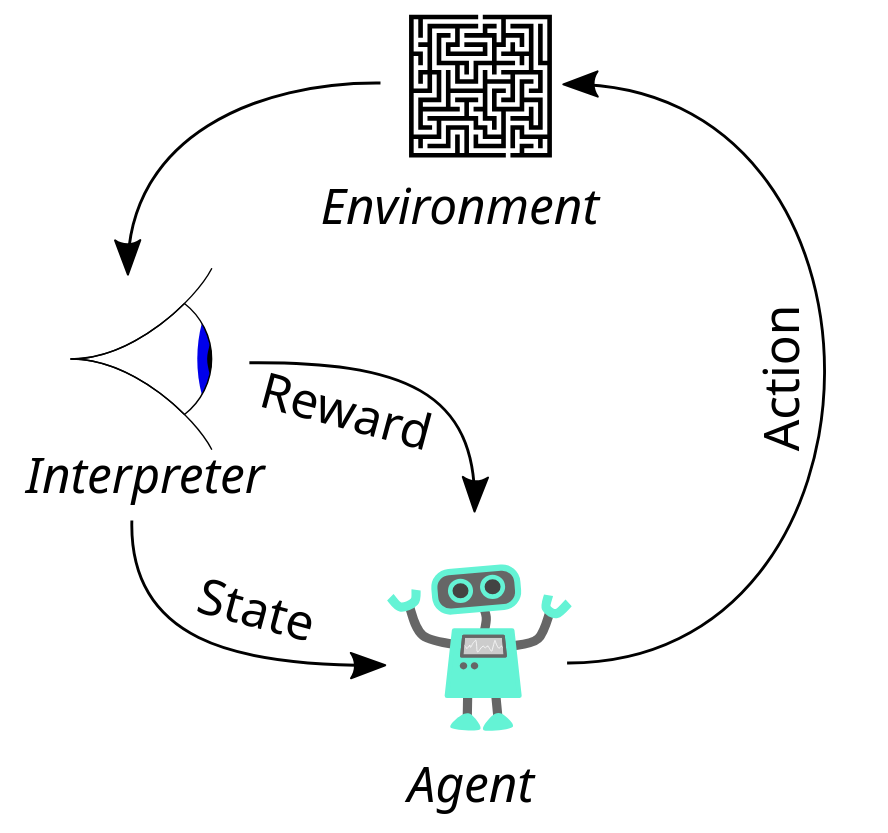
\includegraphics[width=\textwidth]{pictures/Reinforcement_learning_diagram.png}
        \caption{Typowa struktura scenariusza uczenia przez wzmacnianie \cite{wikipedia_reinforcement_learning}}
    \end{figure}

    \section{Modele Markowa (MDP)}
    Wzory i definicje użyte w tej sekcji zostały zaczerpnięte z książki „Reinforcement Learning: An Introduction” autorstwa Suttona i Barto \cite{sutton2018rl}.
    Markowskie procesy decyzyjne (MDP) są formalizacją problemów decyzyjnych w warunkach niepewności, które zakładają spełnienie własności markowskiej: przyszłość (kolejny stan i otrzymana nagroda) zależy jedynie od bieżącego stanu i akcji, a nie od pełnej historii.
    W modelu MDP kluczowymi elementami są:
    \begin{itemize}
        \item Stany i akcje - agent w chwili \( t \) obserwuje stan \( S_t \) ze zbioru stanów \( S \), a następnie wybiera akcję \( A_t \) z dostępnego zbioru akcji \( A \).
        \item Funkcja przejścia i nagród - po wykonaniu akcji \( A_t \) w stanie \( S_t \) agent przechodzi do stanu \( S_{t+1} \) i otrzymuje nagrodę \( R_{t+1} \). Oba te elemenety opisuje funkcja:
        \begin{equation}
        p(s',r|s,a) = P(S_{t+1} = s', R_{t+1} = r | S_t = s, A_t = a).
        \end{equation}
        Dzięki temu wiadomo, z jakim prawdopodobieństwem przy danej akcji w stanie \( s \) agent znajdzie się w stanie \( s' \) oraz jaką otrzyma wtedy nagrodę \( r \).
        \item Oczekiwana nagroda - bardzo często zamiast śledzić cały rozkład nagród, pracuje się z wartością oczekiwaną natychmiastowej nagrody:
        \begin{equation}
        r(s,a) = E[R_{t+1} | S_t = s, A_t = a] = \sum_{s',r} r p(s',r|s,a).
        \end{equation}
        Innymi słowy, jest to średnia nagroda, jakiej agent może oczekiwać w momencie przejścia ze stanu \( s \) do \( s' \) przy akcji \( a \).
        \item Współczynnik dyskontowania - aby modelować długofalowe konsekwencje podejmowanych decyzji, wprowadza się współczynnik \( \gamma \in [0,1] \). Określa on, jak silnie agent ceni przyszłe nagrody w porównaniu z bieżącymi. Gdy \( \gamma = 0 \), agent skupia się wyłącznie na nagrodach natychmiastowych, a gdy \( \gamma \) jest bliskie 1, uwzględnia głównie wpływ aktualnej decyzji na dalszą przyszłość.
    \end{itemize}
    \textbf{Skumulowana nagroda} \\ \\ 
    Dla każdego epizodu w uczeniu przez wzmacnianie definiuje się skumulowaną nagrodę w chwili \( t \) następująco:
    \begin{equation}
    G_t = R_{t+1} + \gamma R_{t+2} + ... = \sum_{k=0}^{\infty} \gamma^k R_{t+k+1}, 
    \end{equation}
    Gdzie:
    \begin{itemize}
        \item \( G_t \) - całkowita (skumulowana) wartość nagród, którą agent otrzymuje od chwili \( t \) aż do zakończenia epizodu,
        \item \( \gamma \) - współczynnik dyskontowania z przedziału \( [0,1] \), który wyznacza, jak bardzo agent ceni przyszłe nagrody w stosunku do natychmiastowych.
        Na przykład:
        \begin{itemize}
            \item dla \( \gamma = 0 \), agent skupia się wyłącznie na nagrodach natychmiastowych,
            \item gdy \( \gamma \) jest blisko 1, agent korzysta z długoterminowych strategii, co może przyniać się do bardziej sensownych akcji,
        \end{itemize}
        \item \( R_{t+k+1} \) - nagroda otrzymana przez agenta w kroku czasowym \( t + k + 1 \). Są to nagrody będące sygnałami zwrotnymi otrzymanymi
        od środowiska, mające na celu informowanie agenta o jakości jego działań,
        \item \( k \) - indeks czasowy, który określa zasięg możliwości przyszłych decyzji agenta, dzięki któremu jest w stanie obliczyć skumulowaną nagrodę.
    \end{itemize}
    Skumulowana nagroda \( G_t \) jest ma kluczowe znaczenie w uczeniu przez wzmacnianie, ponieważ określa ocenę jakości działań agenta. Stanowi ona podstawy cel, który agent stara się 
    maksymalizować poprzez optymalny wybór akcji.
    \\ \\ 
    \textbf{Funkcje wartości i algorytmy uczenia}
    \\ \\ 
    Funkcje wartości stanowią fundament dla wielu algorytmów uczenia przez wzmacnianie, umożliwiając precyzyjną ocenę jakości działań agenta oraz przewidywanie długoterminowych rezultatów podejmowanych decyzji. Poniżej przedstawiono szczegółowe definicje tych funkcji oraz ich zastosowanie w kontekście najważniejszych algorytmów uczenia przez wzmacnianie.
    \begin{itemize}
        \item Funkcja wartości stanu \( V_\pi(s) \) - oczekiwana skumulowana nagroda przy założeniu, że agent znajduje się w stanie \( s \) i przestrzega polityki \( \pi \):
        \begin{equation}
        V_\pi(s) = E_\pi[G_t|S_t=s].
        \end{equation}
        \item Funkcja wartości akcji \( Q_\pi(s,a) \) - oczekiwana skumulowana nagroda przy wykonaniu akcji \( a \) w stanie \( s \), a następnie kontynuacji zgodnie z polityką \( \pi \):
        \begin{equation}
        Q_\pi(s,a) = E_\pi[G_t|S_t=s,A_t=a] .
        \end{equation}
    \end{itemize}
    W podejściu Q-learning następuje iteracyjna aktualizacja wartości \( Q \) w celu wyznaczenia optymalnej polityki,
    natomiast w metodach typu aktor-krytyk (np. A2C) równocześnie modyfikuje się politykę (aktor) i funkcję wartości (krytyk).
    \\ \\ 
    \textbf{Przykład dla gry Pong}
    \\ \\ 
    W celu zilustrowania pojęcia skumulowanej nagrody można rozważyć epizod w grze Pong (patrz sekcja 5.1.1), w której agent otrzymuje w kolejnych krokach czasowych następujące nagrody:    \begin{itemize}
        \item \( r_1 = +1 \) (zdobycie punktu),
        \item \( r_2 = -1 \) (utrata punktu),
        \item \( r_3 = +1 \),
        \item \( r_4 = +1 \),
        \item \( r_5 = -1 \).
    \end{itemize}
    Zakładając że \( \gamma = 0.9 \), wtedy skumulowana nagroda \( G_0 \) zaczynając od chwili \( t = 0 \) będzie obliczana jako:
    \[ G_0 = \gamma^0r_1 + \gamma^1r_2 + \gamma^2r_3 + \gamma^3r_4 + \gamma^4r_5 + ... \]
    \[ G_0 = 1 * 1 + 0.9 * (-1) + 0.9^2 * 1 + 0.9^3 * 1 + 0.9^4 * (-1) + ... \]
    \[ G_0 = 1 - 0.9 + 0.81 + 0.729 - 0.6561 + ... \]
    Maksymalizacja tej sumy wymusza na agencie podejmowanie decyzji zapewniających możliwie największy zysk nie tylko w bieżącym kroku, lecz także w dalszych etapach rozgrywki.
    \section{Równanie Bellmana}
    Wzory i definicje użyte w tej sekcji zostały zaczerpnięte z książki „Reinforcement Learning: An Introduction” autorstwa Suttona i Barto \cite{sutton2018rl}.
    Równanie Bellmana pełni kluczową rolę w teorii uczenia przez wzmacnianie, umożliwiając sformalizowanie zależności między wartościami stanów a podejmowanymi akcjami.
    Używane jest głównie do iteracyjnego obliczania wartości funkcji stanów i akcji, co stanowi fundament wielu algorytmów. 
    Jak zauważyli Sutton i Barto, równanie Bellmana stanowi podstawę dla większości algorytmów uczenia przez wzmacnianie, ponieważ pozwala na efektywne obliczanie wartości stanów i akcji poprzez iteracyjne aktualizacje.
    \subsection{Równanie Bellmana dla funkcji wartości stanu \( V_\pi(s) \)}
    Funkcja wartości stanu \( V_\pi(s) \) wyraża oczekiwaną sumę zdyskontowanych nagród, jakie agent może uzyskać, rozpoczynając od stanu \( s \) i postępując zgodnie z polityką \( \pi \). 
    Równanie Bellmana w tym kontekście ma postać:
    \begin{equation}
    V_\pi(s) = E_\pi[R_{t+1} + \gamma G_{t+1}|S_t = s] = \sum_{a} \pi(a|s) \sum_{s',r} p(s',r|s,a) (r + \gamma V_\pi(s')),
    \end{equation}
    gdzie:
    \begin{itemize}
        \item \( V_\pi(s) \) - Funckja stanu wartości dla polityki \( \pi \), określająca sumę zdyskontowanych nagród od stanu \( s \),
        \item \( E_\pi \) - wartość oczekiwana względem rozkładu wyznaczonego przez politykę \( \pi \),
        \item \( R_{t+1} \) - nagroda otrzymywana po przejściu do stanu \( S_{t+1} \) w wyniku podjęcia akcji zgodnej z \( \pi \), 
        \item \( \gamma \) - Współczynnik dyskonotwania z przedziału \( [0,1] \),
        \item \( S_{t+1} \) - Stan osiągnięty po wykonaniu akcji w stanie \( s \).
    \end{itemize}
    Równanie to można interpretować poprzez równość wartości stanu \( s \) a oczekiwanej nagrody otrzymanej po przejściu do kolejnego stanu plus zdyskontowanej wartości nowego stanu,
    zakładając, iż agent działa zgodnie z polityką \( \pi \).
    \subsection{Równanie Bellmana dla funkcji wartości akcji \( Q_\pi(s,a) \)}
    Funkcja wartości akcji \( Q_\pi(s,a) \) reprezentuje oczekiwaną sumę zdyskontowanych nagród, uzyskiwanych przez agenta w sytuacji, gdy w stanie \( s \) podjęta zostanie akcja \( a \), a w kolejnych krokach zastosowana zostanie polityka \( \pi \). Odpowiednie równanie Bellmana ma postać:
    \begin{align}
    Q_\pi(s,a) = E_\pi[R_{t+1} + \gamma G_{t+1}|S_t = s, A_t = a] \notag
    \\= \sum_{a} \pi(a|s) \sum_{s',r} p(s',r|s,a)(r + \gamma \sum_{a} \pi(a|s)Q_\pi(s',a'))
    \end{align}
    Zgodnie z tym równaniem wartość akcji \( a \) w stanie \( s \) zależy od natychmiastowej nagrody oraz zdyskontowanej wartości przyszłych akcji, które zostaną wybrane zgodnie z polityką \( \pi \).
    \subsection{Równanie Bellmana dla polityki optymalnej \( V_*(s) \) i \( Q_*(s,a) \)}
    Polityka optymalna \( \pi_* \) maksymalizuje funkcję wartości stanu. Oznacza to, że:
    \begin{equation}
    V_*(s) = \max_{\pi} V_{\pi}(s)
    \end{equation}
    Równanie Bellmana dla optymalnej funkcji wartości stanu może zostać zapisane w postaci:
    \begin{equation}
    V_*(s) = \max_{a} E[R_{t+1} + \gamma V_*(S_{t+1})|S_t = s, A_t = a] = 
    \max_{a} \sum_{s',r} p(s',r|s,a)(r + \gamma V_*(s'))
    \end{equation}
    Analogicznie, optymalna funkcja wartości akcji wyraża się wzorem:
    \begin{align}
    Q_*(s,a) = E[R_{t+1} + \gamma \max_{a'} Q_*(S_{t+1},a')|S_t = s, A_t = a] \notag
    \\= \sum_{s',r} p(s',r|s,a)(r + \gamma \max_{a'} Q_*(s',a'))
    \end{align}
    Powyższe równania można interpretować następująco:
    \begin{itemize}
        \item \( V_*(s) \) - najlepsza możliwa wastość stanu \( s \), uzyskana poprzez wybór najlepszej akcji.
        \item \( Q_*(s,a) \) - najlepsza możliwa wartość akcji \( a \) w stanie \( s \), przy założeniu dalszego postępowania według optymalnej strategii.
    \end{itemize}
    Opisane zależności leżą u podstaw algorytmów takich jak Value Iteration czy Q-learning, które dążą do znalezienia polityki maksymalizującej skumulowaną nagrodę.
    \subsection{Metoda iteracji wartości}
    Metoda iteracji wartości to algorytm, który pozwala na iteracyjną aktualizację funkcji wartości stanu \( V(s) \) zgodnie z równaniem Bellmana dla optymalnej polityki, do momentu osiągnięcia zbieżności.
    \\ Składa się ona z poniższych kroków:
    \begin{enumerate}
        \item Zainicjalizuj wszystkie stany \( V_i \) z pewnymi wartościami początkowymi. Zawyczaj \( V(s) = 0 \) dla wszystkich \( s \in S \).
        \item Dla każdego stanu \( s \in S \) w procesie decyzyjnym Markowa wykonaj aktualizacje:
        \begin{equation}
        V(s) \leftarrow \max_a \sum_{s',r} p(s',r|s,a)[r + \gamma V(s')]
        \end{equation}
        \item Powtarzaj poprzedni krok poprzez wykonanie wielu iteracji do momentu gdy maksymalna zmiana \( V(s) \) jest mniejsza niż zadany próg. 
    \end{enumerate}
    \subsection{Metoda iteracji polityki}
    Metoda iteracji polityki to algorytm składający się z dwóch głównych kroków: ewaluacji polityki i jej ulepszania. Jego szczegóły są następujące:
    \begin{enumerate} 
        \item Zainicjalizuj początkową politykę \( \pi(s) \) oraz \( V(s) \).
        \item Oblicz wartość \( V(s) \) dla bierzącej polityki \( \pi \) za pomocą poniższego wzoru:
        \begin{equation}
        V(s) \leftarrow \sum_{s',r} p(s',r|s,\pi(s))(r + \gamma V(s')).
        \end{equation}
        \item ulepszenie polityki poprzez wybór akcji \( a \) maksymalizującej wartość oczekiwaną dla każdego stanu \( s \) za pomocą poniższego wzoru:
        \begin{equation}
        pi'(s) = \arg\max_{a} \sum_{s',r} p(s',r|s,a) [r + \gamma V(s')].
        \end{equation}
        \item Jeżeli \( \pi' = \pi \), kończy się proces w przeciwnym wypadku ustaw \( \pi \leftarrow \pi' \) i ponów kroki 2-3.
    \end{enumerate}
    \section{Metoda entropii krzyżowej w uczeniu przez wzmacnianie}
    Wzory i definicje użyte w tej sekcji zostały zaczerpnięte z książki „Deep Reinforcement Learning Hands-On.” autorstwa Maxima Lapana \cite{lapan2020deep}.
    Entropia krzyżowa jest miarą różnicy pomiędzy dwoma rozkładami prawdopodobieństwa. W kontekście uczenia przez wzmacnianie bywa wykorzystywana do oceny jakości nowej polityki \( \pi_{new} (a|s) \) względem idealnego rozkładu akcji, który ma maksymalizować skumulowaną nagrodę. Definicja entropii krzyżowej pomiędzy rozkładami \( p(a) \) i \( q(a) \) ma postać:
    \begin{equation}
    H(p,q) = - \sum_{a \in A} p(a) log(q(a))
    \end{equation}
    gdzie:
    \begin{itemize}
        \item \( p(a) \) - rozkład prawdopodobieństwa akcji \( a \) według starej polityki \( \pi_{old}(a|s) \).
        \item \( q(a) \) - rozkład prawdopodobieństwa akcji \( a \) według nowej polityki \( \pi_{new} (a|s) \).
    \end{itemize} 
    \subsection{Twierdzenie o próbkowaniu istotnościowym}
    Próbkowanie istotnościowe pozwala na wykorzystanie próbek pochodzących z pewnego rozkładu prawdopodobieństwa w celu oszacowania wartości oczekiwanej funkcji definiowanej względem innego rozkładu. W uczeniu przez wzmacnianie z próbkowaniem istotnościowym ma się do czynienia np. wtedy, gdy dane są zbierane na podstawie starej polityki \( \pi_{old}(a|s) \), zaś celem jest szacowanie wartości dla nowej polityki \( \pi_{new} (a|s) \).
    \begin{theorem}[O próbkowaniu istotnościowym]
    \begin{equation}
    E_{x \sim p(x)} [H(x)] = \int_{x} p(x)H(x) dx = \int_{x} q(x) \frac{p(x)}{q(x)} H(x) dx = E_{x \sim q(x)} [\frac{p(x)}{q(x)}H(x)]
    \end{equation}
    \end{theorem}
    gdzie:
    \begin{itemize}
        \item \( p(x) \) - rozkład próbkowania (np. stara polityka)
        \item \( q(x) \) - rozkład docelowy (np. nowa polityka)
        \item \( H(x) \) - funkcja entropii w stanie \( x \) często definiowana jako:
        \begin{equation}
        H(\pi) = - \sum_{a \in A} \pi(a|s)log(\pi(a|s)) 
        \end{equation}
    \end{itemize}
    \subsection{Dywergencja Kullbacka-Leiblera}
    Dywergencja Kullbacka-Leiblera (KL) mierzy odległość między dwoma rozkładami prawdopodobieństwa \( p(x) \) i \( q(x) \). W uczeniu przez wzmacnianie może służyć do kontrolowania, jak bardzo nowa polityka różni się od starej, co pomaga zapobiegać gwałtownym zmianom w trakcie treningu. Definicję KL przedstawia równanie:
    \begin{equation}
    KL(p(x) || q(x)) = \sum_{x} p(x) \frac{p(x)}{q(x)}.
    \end{equation}
    W kontekście uczenia przez wzmacnianie:
    \begin{equation}
    KL(\pi_{old}(a|s) || \pi_{new}(a|s)) = \sum_{a} \pi_{old}(a|s) log(\frac{\pi_{old}(a|s)}{\pi_{new}(a|s)})
    \end{equation}
    Dywergencja Kullbacka-Leiblera jest używana do:
    \begin{itemize}
        \item regularizacji polityki - ogranicza stopień zmiany między starą a nową polityką, co pomaga uniknąć niestabilnych lub niepożądanych zachowań podczas trenowania,
        \item kontrola eksploracji - wspiera utrzymanie równowagi między eksploracją nowych akcji a wykorzystywaniem już poznanych strategii.
    \end{itemize}
    \section{Implementacjia wybranych algorytmów uczenia przez wzmacnianie}
    Istnieje wiele algorytmów wykorzystywanych w uczeniu przez wzmacnianie \cite{sutton2018rl}, a konkretny wybór zależy głównie od charakterystyki środowiska oraz rodzaju problemu. Zwyczajowo dzieli się je na trzy główne kategorie:
    \begin{itemize}
        \item algorytmy optymalizujące wartości (Value Optimization),
        \item algorytmy optymalizujące politykę (Policy Optimization),
        \item algorytmy imitacyjne (imitation).
    \end{itemize}
    \section{Klasyfikacja algorytmów uczenia przez wzmacnianie}
    \subsection{Algorytmy optymalizujące wartości}
    W algorytmach tej grupy zasadniczym celem jest wyuczenie funkcji wartości, która pozwala oceniać jakości stanów lub akcji w danym czasie. Przykładem jest algorytm Q-Learning, koncentrujący się na wyznaczaniu funkcji \( Q(s,a) \) (patrz wzór (3.5)), wyrażającej oczekiwaną sumę zdyskontowanych nagród po wykonaniu akcji \( a \) w stanie \( s \) przy założeniu postępowania według polityki optymalnej. Inne popularne algorytmy to: Deep Q-Learning (DQN) \cite{mnih2015dqn}, double DQN \cite{vanhasselt2016deep}, dueling DQN. \cite{wang2016dueling}
    \subsection{Algorytmy optymalizujące politkę}
    Podejście to polega na bezpośredniej optymalizacji polityki, czyli reguły wyboru akcji w każdym stanie \cite{sutton2018rl}. Zamiast modelować funkcję wartości, dąży się do znalezienia strategii maksymalizującej oczekiwaną sumę nagród.
    \\ \textbf{Przykładowe algorytmy:}
    \begin{itemize}
        \item Policy Gradient Methods (REINFORCE) \cite{williams1992simple}
        \item Advantage Actor-Critic (A2C) \cite{konda2000actor}
        \item Asynchronous Advantage Actor-Critic (A3C) \cite{mnih2016a3c}
        \item Proximal Policy Optimization (PPO) \cite{schulman2017proximal}
    \end{itemize}
    \subsection{Algorytmy imitacyjne}
    W podejściu imitacyjnym algorytm wzoruje się na działaniach eksperta (tzw. expert policy) i uczy się replikowania jego skutecznych zachowań bez konieczności przeprowadzania pełnej eksploracji środowiska.
    \\ \textbf{Przykładowe algorytmy:}
    \begin{itemize}
        \item Behavioral Cloning \cite{bain1995framework}
        \item Inverse Reinforcement Learning (IRL) \cite{ng2000algorithms}
        \item Generative Adversarial Imitation Learning (GAIL) \cite{ho2016generative}
    \end{itemize}
    \section{Wybór algorytmów do implementacji}
    W ramach realizowanego projektu postanowiono skupić się na algorytmach wywodzących się z dwóch pierwszych grup, a więc Deep Q-Learning (DQN) oraz Advantage Actor-Critic (A2C). Wybór wynika głównie z charakteru wybranego środowiska i celów badawczych związanych z grą Pong.
    \subsection{Dlaczego odrzucono klasyczną metodę Q-Learning?}
    Klasyczny Q-Learning, mimo że stanowi fundament uczenia przez wzmacnianie, bywa niewystarczający w bardziej złożonych środowiskach, na przykład w grach wideo. Istnieje kilka istotnych ograniczeń tej metody:
    \begin{itemize}
        \item wysoka wymiarowość przestrzeni stanów - gry Atari, w tym Pong, generują wielowymiarowe dane wejściowe, przez co tablicowe podejście do Q-funkcji staje się niepraktyczne,
        \item brak generalizacji - tablicowa wersja Q-Learningu nie potrafi przekładać wiedzy z jednych stanów na inne, co ogranicza szybkość i skuteczność nauki,
        \item trudność z eksploracją - klasowa metoda Q-Learningu wymaga rozbudowanej fazy eksploracyjnej, co powoduje duże zapotrzebowanie na czas i zasoby,
        \item brak stabilności procesu uczenia - w dużych, dynamicznych przestrzeniach stanów uczenie metodą Q-Learning potrafi ulegać częstym fluktuacjom lub nawet nie osiągać zbieżności. 
    \end{itemize}
    Z tych względów zdecydowano się na zastosowanie algorytmów, które wykorzystują sieci neuronowe w roli aproksymatora funkcji wartości. Tego rodzaju rozwiązania pozwalają na skuteczniejsze radzenie sobie z wysokowymiarowymi danymi. \cite{mnih2015nature}
    \section{Deep Q-Learning (DQN)}
    Deep Q-Learning (DQN) stanowi rozwinięcie klasycznej metody Q-Learning, w którym w miejsce tablicowej reprezentacji funkcji \( Q(s,a) \) wykorzystuje się głęboką sieć neuronową. Pozwala to agentowi na efektywną naukę w środowiskach cechujących się złożonymi i licznie występującymi stanami.
    \subsection{Architektura modelu}
    Podstawą algorytmu DQN jest sieć neuronowa pełniąca funkcję aproksymatora wartości \( Q(s,a;\theta) \). Najistotniejsze elementy tej architektury to \cite{mnih2015nature}:
    \begin{itemize}
        \item Sieć Q - aproksymuje funkcję \( Q \). Otrzymuje na wejściu reprezentację stanu (np. wycinek obrazu) i generuje estymowane wartości \( Q \) dla każdej możliwej akcji w tym stanie.
        \item Sieć docelowa - kopia sieci \( Q \), aktualizowana rzadziej niż zasadnicza sieć \( Q \). Ma to na celu stabilizację treningu, ponieważ ogranicza wzajemne sprzężenie pomiędzy siecią \( Q \) a docelową wartością przy obliczaniu błędu.
        \item Bufor doświadczeń - przechowuje pary \( ( s_t, a_t, r_{t+1}, s_{t+1}) \), które pochodzą z kolejnych interakcji agenta ze środowiskiem. W trakcie uczenia próbki losuje się z bufora, dzięki czemu redukuje się korelację między kolejnymi próbkami.
    \end{itemize}
    \subsection{Proces treningu algorytmu DQN}
    Trening DQN składa się z następujących kroków \cite{lapan2020deep}:
    \begin{enumerate}
        \item Inicjalizacja:
        \begin{itemize}
            \item Sieć Q - losowa inicjalizacja wag \( \theta \).
            \item Sieć docelowa - ustawienie wag \( \theta' \) równych \( \theta \),
            \item Bufor doświadczeń - utworzenie pustej struktury do magazynowania próbek \( (s,a,r,s') \).
        \end{itemize}
        \item Wybór akcji (tzw. strategia \( \epsilon \)-greedy): \\
        Akcja \( a_t \) w stanie \( s_t \) jest wybierana w sposób probabilistyczny:
        \[
        a_t =
        \begin{cases} 
        \text{losowa akcja} & \text{z prawdopodobieństwem } \epsilon, \\
        \arg\max\limits_{a} Q(s_t, a; \theta) & \text{z prawdopodobieństwem } 1 - \epsilon.
        \end{cases}
        \]
        \item Interakcja ze środowiskiem:
        \begin{itemize}
            \item wykonanie akcji \( a_t \), otrzymanie nagrody \( r_{t+1} \) i przejście do nowego stanu \( s_{t+1} \)
            \item zapis przejścia \( s_t, a_t, r_{t+1}, s_{t+1} \)  w buforze.
        \end{itemize}
        \item Pobranie próbek z bufora:
        \begin{itemize}
            \item losowanie niewielkiej partii (mini-batch) przejść \( {(s_i, a_i, r_i, s'_i)} \)
            \item jeżeli epizod zakończył się w tym kroku, to dla każdego z przejść oblicz wartość docelową \( y = r \). W przeciwnym razie użyj 
            wzoru \( y_i = r_i + \gamma \max_{a'} Q(s'_i, a'_i; \theta') \), gdzie \( \theta' \) to wagi sieci docelowej.
        \end{itemize}
        \item Obliczanie straty (np. błędu średniokwadratowego):
        \begin{equation}
        \mathcal{L}(\theta) = \frac{1}{N} \sum_{i}(Q(s_i,a_i;\theta)-y_i)^2 
        \end{equation}
        \item Aktualizacja wartość \( Q(s,a) \) za pomocą algorytmu stochastycznego spadku wzdłuż gradientu poprzez minimalizacje straty w odniesieniu do parametrów modelu.
        \item Aktualizacja wag sieci \( Q \) - Przypisanie \( \theta \) do \( \theta' \) po ustalonej liczbnie kroków, co stabilizuje proces uczenia.
        \item Powtarzanie kroków 2-7 do momentu osiągnięcia stabilnych wyników.
    \end{enumerate}
    \subsection{Przykładowa architektura sieci Q dla DQN}
    \begin{itemize}
        \item Warstwa wejściowa - wejście w postaci obrazu o rozmiarze 84x84 pikseli z 4 kanałami
        \item Pierwsza warstwa konwolucyjna - 32 filtry, rozmiar jądra 8x8, stride 4, aktywacja ReLU.
        \item Druga warstwa konwolucyjna - 64 filtry, rozmiar jądra 4x4, stride 2, aktywacja ReLU.
        \item Trzecia warstwa konwolucyjna - 64 filtry, rozmiar jądra 3x3, stride 1, aktywacja ReLU.
        \item Warstwa w pełni połączona - 512 neuronów, aktywacja ReLU.
        \item Warstwa wyjściowa - liczbna neronów jest równa liczbie dostępnych akcji w środowisku, bez wykorzystania funkcji aktywacji
    \end{itemize}
    \section{Advantage Actor-Critic (A2C)}
    Advantage Actor-Critc (A2C) to metoda, która łączy w sobie zalety metod opartych na polityce i opartych na wartściach \cite{mnih2016a3c} \cite{stable_baselines_a2c}.
    Pozwala ona na zminiejszczenie wariancji poprzez uzależnienie punktu odniesienia od stanu. Nagrodę można przedstawić
    jako wartość stanu plus przewaga akcji: \( Q(s,a) = V(s) + A(s,a) \). A2C działa na zasadzie wykorzystania dwóch odzielnych
    sieci nauronowych: aktora odpowiedzialnego za wybór akcji oraz krytyka oceniającego jakość stanu lub poprawność wyboru akcji, dostarczając użytecznych sygnałów uczących.
    \subsection{Architektura modelu}
    W modelu A2C zwykle wykorzystuje się jedną sieć neuronową (z ewentualnie współdzielonymi warstwami początkowymi), która rozgałęzia się na dwie części wyjściowe - aktora i krytyka:
    \begin{enumerate}
        \item Część współdzielona:
        \begin{itemize}
            \item Warstwa wejściowa - przyjmuje stan środowiska s. W przypadku gier Atari jest to np. znormalizowany obraz w skali szarości o wymiarach 84 x 84 piksele. W przypadku środowisk wektorowych warstwa wejściowa może mieć postać zwykłego wektora cech.
            \item Warstwy ukryte - zwykle stosuje się kilka warstw konwolucyjnych do wyodrębniania cech z obrazu. Przy środowiskach o wejściu wektorowym wystarczające mogą być 2 lub 3 warstwy w pełni połączone.
            \item Wspólna reprezentacja cech - wyjście z warstw konwolucyjnych stanowi rdzeń, współdzielony zarówno przez aktora jak i krytyka. Dzięki temu aktor i krytyk uczą się wspólnej reprezentacji stanu, co często poprawia efektywność i stabilność trenowania.
        \end{itemize}
        \item Sieć aktora - odpowiada za generowanie rozkładu prawdopodobieństwa akcji \( \pi(a,s) \) w danym stanie \( s \):
        \begin{itemize}
            \item Warstwa wejściowa - przyjmuje jako dane wejściowe stan środowiska.
            \item Warstwy ukryte - zawierają kilka warstw połączonych lub konwolucyjnych, których celem jest ekstrakcja cech oraz transformacja informacji.
            \item Warstwa wyjściowa - zwykle kończy się funkcją softmax, wyprowadzającą prawdopodobieństwo każdej możliwej akcji:
            \begin{equation}
            \pi(a|s) = \frac{exp(f(a,s))}{\sum_{a'}exp(f(a',s))},
            \end{equation}
            gdzie \( f(a,s) \) jest wynikiem ostatniej warstwy sieci aktora.
        \end{itemize}
        \item Sieć Krytyka - jest odpowiedzialna za szacowanie wartości stanu \( V(s) \) (a także przewagi \( A(s,a) \), jeśli zostanie odpowiednio zaprojektowana). Ma to kluczowe znaczenie przy dostarczaniu trafnej oceny jakości działań aktora.
        \item Warstwa wejściowa - przyjmuje stan środowiska jako dane wejściowe, podobnie jak sieć aktora, czasem dodaje się też dodatkową warstwę połączoną.
        \item Warstwa ukryta - z reguły zbliżone do tych w sieci aktora, przetwarzające dane wejściowe.
        \item Warstwa wyjściowa - ma postać pojedynczej jednostki (neuronu), której wartość numeryczna reprezentuje \( V(s) \), czyli estymowaną wartość stanu:
        \begin{equation}
        V(s) = f_{critic}(s).
        \end{equation}    
    \end{enumerate}
    \subsection{Proces treningu algorytmu A2C}
    Poniżej przedstawiono zarys treningu metody A2C, uwzględniający interakcję agenta ze środowiskiem, gromadzenie doświadczeń, obliczanie przewagi oraz aktualizację parametrów \cite{lapan2020deep}. 
    \begin{enumerate}
        \item Inicjalizacja - nadanie losowych wartości parametrom \( \theta \). Zwykle wyróżnia się: 
        \begin{itemize}
            \item \( \theta_{\pi} \) - parametry sieci aktora,
            \item  \( \theta_v \) - parametry sieci krytyka.
        \end{itemize}
        \item Wykonanie N kroków przy użyciu bierzącej polityki \( \pi_{\theta_\pi} \), Agent wykonuje \( N \) kroków w środowisku. Dla każdego kroku \( t \) zapisywane są: stan \( s_t \), akcja \( a_t \) oraz nagroda \( r_t \).
        \item Obliczenie wartości końcowej R - jeżeli epizod uległ zakończeniu, przyjmuje się \( R = 0 \). W przeciwnym wypadku oblicza się wartość stanu końcowego \(s_{t} \) przy użyciu sieci wartości: 
        \begin{equation}
        R = V_{\theta_v}(s_{t}).
        \end{equation}
        W przypadku zakończenia epizodu, na przykład gdy gra się kończy, przerywamy zbieranie danych wcześniej.
        \item Przetwarzanie wstecz i aktualizacja parametrów - 
        rozważając kroki wstecz od \( i = t-1, ..., t_{start} \), aktualizuje się wartość \( R \):
        \begin{equation}
        R \leftarrow r_i + \gamma R 
        \end{equation}
        Następnie należy aktualizować gradienty aktora i krytyka:
        \begin{itemize}
            \item gradient polityki:
            \begin{equation}
            \partial \theta_\pi \leftarrow \partial \theta_\pi +  \nabla_{\theta_\pi} log \pi_{\theta_\pi} (a_i|s_i) (R-V_{\theta_v}(s_i)),
            \end{equation}
            \item gradient wartości:
            \begin{equation}
            \partial \theta_v \leftarrow \partial \theta_v + \frac{\partial(R-V_{\theta_v}(s_i))^2}{\partial \theta_v}
            \end{equation}
        \end{itemize}
        Sumujemy powyższe gradienty dla aktora i krytyka.
        \item Aktualizacja parametrów sieci wykorzystując zsumowane gradienty. Należy przesunąć się w kierunku gradientów polityki \( \partial \theta_\pi \) (maksymalizacja polityki) oraz w kierunku przeciwnym do gradientów wartości \( \partial \theta_v \) (minimalizacja błędu wartości).
        \item Powtórzenie kroków 2-5 do momentu osiągnięcia konwergencji lub uzyskania założonych winików.
    \end{enumerate}
    \section{Eksperymenty i analiza wyników}
    \section{Konfiguracja środowiska testowego}
    Głównym celem badań jest przetestowanie wybranych algorytmów uczenia przez wzmacnianie w prostej grze wydanej przez Atari \cite{bellemare2013arcade}. Z tego powodu podjęto decyzję o wyborze gry Pong jako środowiska testowego. W celu uproszczenia procesu implementacji oraz uniknięcia nadmiarowego kodu zastosowano bibliotekę Gymnasium \cite{gymnasium2025}, zapewniającej ujednolicony interfejs API umożliwiający interakcję agenta z otoczeniem.
    \subsection{Środowisk testowe: Pong}
    Pong jest popularną grą wideo wydaną po raz pierwszy przez Atari. Idealnie nadają się do testowania algorytmów uczenia przez wzmacnianie. W projekcie wykrzystano środowisko PongNoFrameskip-v4, dostarczone przez bibliotekę Arcade Learning Environment \cite{bellemare2013arcade}. Wiele algorytmów zostało przetestowanych i wykorzystanych jako benchmark w uczeniu maszynowych ze względu na prostotę implementacji biblioteki. Warto też zwrócić
    uwagę, że Pong wymaga od agenta skutecznego podejmowania decyzji w czasie rzeczywistym przez co nadaje się idealnie do testów.
    \subsection{Charakterystyka środowiska Pong} 
    \begin{itemize}
        \item Stan Środowiska -  stan odzwierciedla aktualny obraz z gry, o wymiarach 210 x 160 x3  (wysokość, szerokość, kanały RGB). W celu zwiększenia efektywności uczenia przeprowadza się wstępne przetwarzanie, zmniejszając rozdzielczość oraz upraszczając dane wejściowe.
        \item Zbiór akcji - dla gry Pong mamy możliwość wykonania trzech akcji: przesunięcie paletki w góre, przesunięcie paletki w dół oraz pozostawienie paletki w miejscu.
        \item Nagrody - sposób przyznawania nagród dla naszego środowiska wyraża się w następujący sposób:
        \begin{description}
        \item +1: agent zdobywa punkt w momencie odbicia piłki w taki sposób aby przeciwnik nie był w stanie jej odbić,
        \item -1: w momencie gdy agent nie zdoła odbić piłki przeciwnik otrzymuje punkt, 
        \item 0: dla pozostałych przypadków np: w trakcie wymiany odbić.
        \end{description}
        \item Warunek końca epizodu - koniec jednego epizodu uczenia następuje w momencie, gdy agent lub jego przeciwnik osiągnie 21 punktów.
        \item Cel agenta - maksymalizacja całkowitej zdyskontowanej nagrody w trakcie jednego epizodu, co jest równoznaczne z wygrywaniem większą liczbą punktów niż przeciwnik.
    \end{itemize}
    \subsection{Język programowania: Python}
    W ramach implementacji algorytmów uczenia przez wzmacnianie zdecydowano się na użycie języka programowania Python \cite{python}. Głównymi aspektami przemawiającym za wybraniem tego języka są przede wszystkim szeroka gama bilbiotek wspierających uczenie przez wzmacnianie (np. Gymnasium \cite{gymnasium2025}, Pytorch \cite{pytorch2025}). Python jest najpopularniejszym językiem stosowanym w dziedzinie sztucznej inteligencji i uczenia przez wzmacnianie. Duża część współczesnych rozwiązań w AI jest implementowana właśnie w Pythonie, co przekłada się na bogate wsparcie społeczności.
    \subsection{Biblioteki wykorzystane do implementacji}
    \begin{itemize}    
        \item Gymnasium \cite{gymnasium2025} - biblioteka stanowiąca standard dla uczenia przez wzmacnianie, służąca do symulacji środowisk. Zastosowaną ją głównie w celu dostarczenia środowiska gry Pong, oraz
        łatwości w zapewnieniu interfejsu dla agenta, który ma mu służyć do interakcji ze środowiskiem. Biblioteka oferuje prostą interakcję z różnymi algorytmami uczenia przez wzmacnianie.
        \item PyTorch \cite{pytorch2025} - pozwala na implementacje złożonych modeli uczenia przez wzmacnianie opartych na sieciach neuronowych za pomocą kilku linijek kodu. 
        PyToch zapewnia dwie wysokopoziomowe funkcję: obliczenia tensorowe z silną akceleracją przy pomocy wykorzystania procesorów graficznych, 
        wykorzystanie głębokich sieci neuronowych zaprojektowanych za pomocą taśmowych systemów automatycznego różnicowania.
        \item OpenCV \cite{opencv2025} - zestaw narzędzi pozwalający na przetwarzanie obrazu oraz widzenie komputerowe. Dzięki wykorzystaniu tej biblioteki jesteśmy w stanie
        osiągnąć szybkie iw wydajne przetwarzanie danych graficznych przed przesłaniem ich do sieci neuronowej. 
    \end{itemize}
    \section{Wyniki dla modelu Deep Q-Learning}
    Model Deep Q-Learning (DQN) został zaimplementowany w celu wytrenowania agenta do gry Pong przy użyciu sieci neuronowej do aproksymacji funkcji \( Q \). Architektura algorytmu opiera się na bibliotekach PyTorch, Gymnasium oraz OpenCV. Dodatkowo środowisko Pong poddano wstępnemu przetwarzaniu (tzw. wrappery), aby usprawnić proces uczenia.
    \newpage
    \subsection{Analiza wykresu nagordy}
    \begin{figure}[htbp]
        \centering
        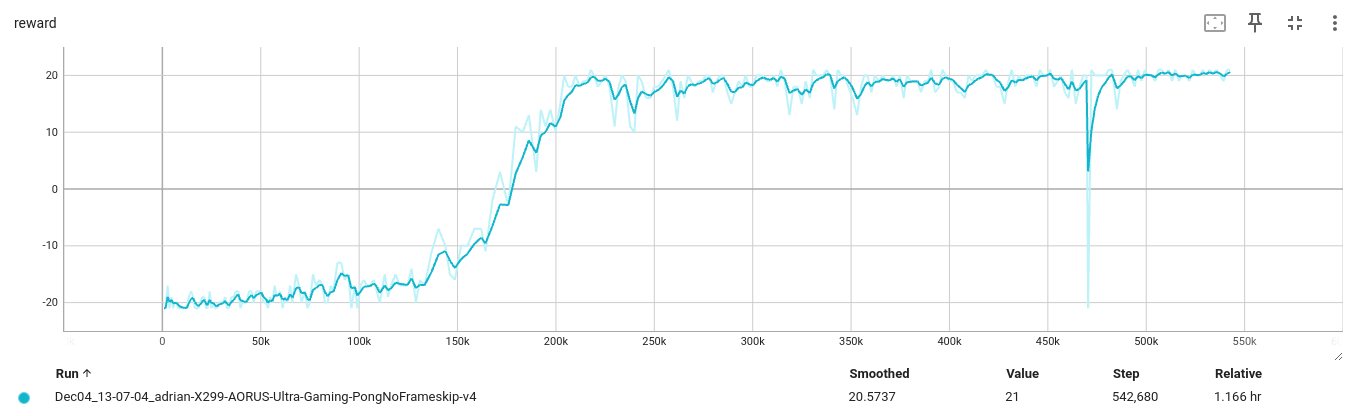
\includegraphics[width=\textwidth]{pictures/DQL_reward.png}
        \caption{Wykres przedstawiający średnią nagrodę modelu DQN}
        \label{fig:etykieta_obrazka}
    \end{figure}
    Widzimy, że na początku treningu agent wykonuje
    losowe ruchy czyli, eksploruje środowisko, co jest adekwatne do otrzymywania nagród na poziomie około -21 (maksymalnej możliwej przegranej). 
    Następnie obserwujemy powolny wzrost wartości nagród, co wskazuje na szukanie podstawowych strategii przez agenta. Po około 100 000 
    krokach treningowych następuje gwałtowny wzrost otrzymywanej średniej nagrody agenta, co wskazuje na stopniową naukę strategii gry.
    W okolicy 175 000 kroków średnia nagroda zaczyna przekraczać punkt 0, co oznacza, że agent zaczyna wygrywać więcej razy w trakcie jednego epizodu gry.
    W momencie około 300 000 kroków można zaobserwować osiągnięcie stopniowej stabilności wyników, zbliżając się do maksymalnej średniej nagrody wynoszącej +21.
    W kolejnych krokach widać niewielkie wahania wyników co jest związane ze stochastyczną naturą dynamicznego środowiska gry Pong.
    Proces treningu został zakończony w ciągu około 540 000 kroków, przy czasie trwania procesu uczenia wynoszącym 1,166 godziny czasu rzeczywistego.
    \subsection{Struktura projektu}
    W niniejszej części przedstawiono uproszczony diagram klas (w notacji UML) ilustrujący kluczowe elementy architektury implementacji algorytmu Deep Q-Learning dla gry Pong. Diagram pokazany na rys. 5.2 zawiera zarówno klasy związane z gromadzeniem i przetwarzaniem danych (m.in. bufor doświadczeń i tak zwane wrappery), jak również samą sieć neuronową (DQN) i logikę podejmowania decyzji przez agenta. Dzięki tak zorganizowanej strukturze możliwa jest wieloetapowa analiza sekwencji obserwowanych stanów w środowisku oraz generowanie akcji w oparciu o metodologie uczenia ze wzmocnieniem.
    \begin{figure}[H]
        \centering
        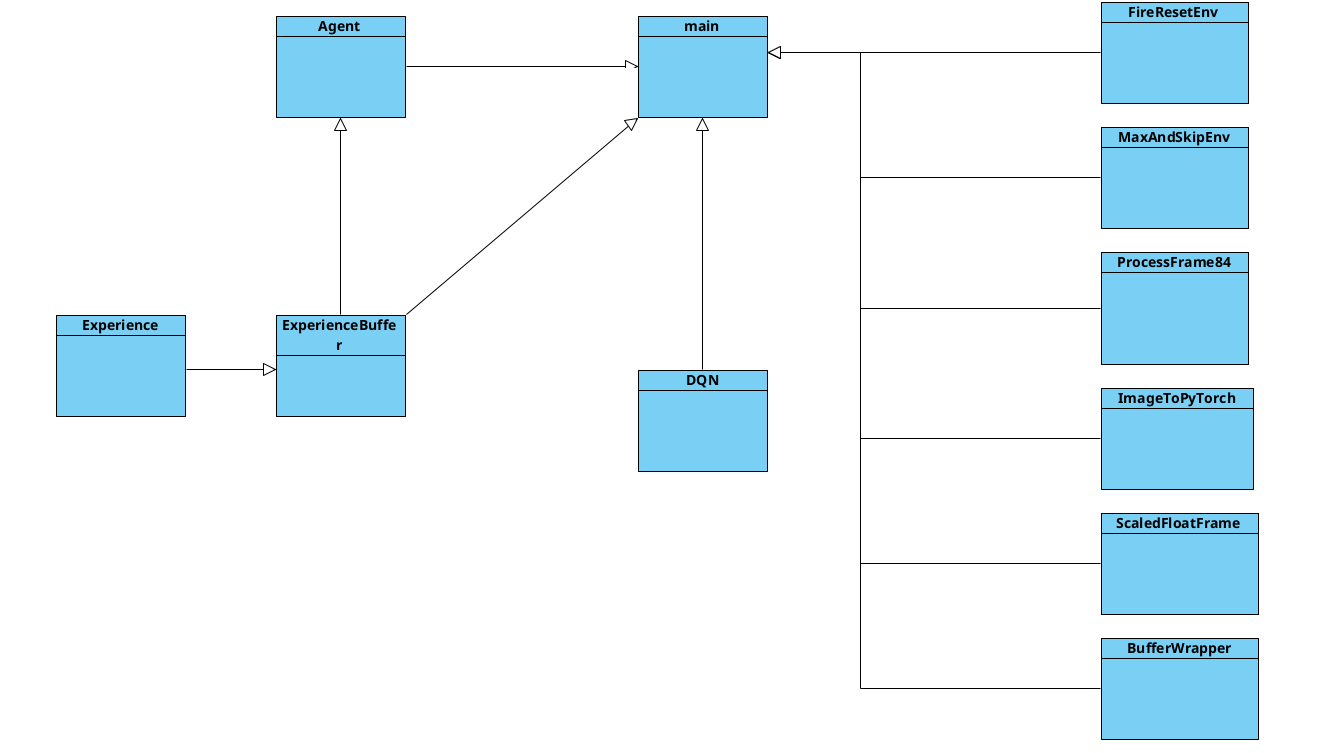
\includegraphics[width=\textwidth]{pictures/DQN_diagram.png}
        \caption{Diagram stuktury projektu}
    \end{figure}
    \begin{itemize}
        \item Main - moduł główny odpowiada za inicjalizację środowiska Pong, wykorzystując dedykowane wrappery ułatwiające proces uczenia. W jego obrębie tworzone są również wszystkie obiekty niezbędne do trenowania modelu: sieć DQN, bufor doświadczeń oraz agent. Moduł zarządza pętlą treningową - w każdej iteracji agent podejmuje akcje w środowisku, kolekcjonuje nowe doświadczenia i przekazuje je dalej do procesu uczenia. Ponadto, w pliku tym ustala się podstawowe hiperparametry (np. współczynnik uczenia, początkowy poziom eksploracji \( \epsilon \) czy rozmiar partii treningowej w buforze doświadczeń) oraz definiuje sposób rejestrowania postępów treningu.
        \item Agent - klasa Agent stanowi łącznik między środowiskiem a siecią Q. Jej zadaniem jest wybór akcji na bazie przyjętej polityki (np. \( \epsilon \)-greedy) oraz monitorowanie bieżącego stanu gry, w tym gromadzenie nagród i informacji o zakończeniu epizodów. Agent organizuje również zapisywanie doświadczeń w buforze, co umożliwia efektywniejsze uczenie modelu w oparciu o różne fragmenty rozgrywki.
        \item ExperienceBuffer - zapewnia strukturę do przechowywania doświadczeń generowanych przez agenta. Dzięki temu możliwe jest wielokrotne wykorzystanie zapisanych informacji podczas uczenia, co wspomaga stabilność procesu treningowego i poprawia jakość nabywanych przez sieć neuronową reprezentacji.
        \item Experience - pojedynczy krok w środowisku (tzw. transition) został zdefiniowany w klasie Experience. Zawiera ona kluczowe dane opisujące stan przed podjęciem akcji, stan po jej wykonaniu, otrzymaną nagrodę oraz informację o ewentualnym zakończeniu epizodu. Każdy obiekt tej klasy wykorzystywany jest następnie przez bufor doświadczeń podczas przygotowywania próbek treningowych dla sieci DQN.
        \item DQN - sieć DQN służy do aproksymacji funkcji Q. W opisywanym projekcie wykorzystano sieć konwolucyjną, zaprojektowaną do analizy sekwencji obrazów pochodzących z rozgrywki. Przetworzone przez sieć dane wejściowe umożliwiają wyznaczenie wartości Q dla wszystkich możliwych akcji. Agent, na podstawie tych wartości, wybiera ruch dążący do maksymalizacji skumulowanej nagrody w dłuższym horyzoncie czasowym.
        \item MaxAndSkipEnv - mechanizm pozwalający pominąć część klatek i jednocześnie zsumować odpowiadające im nagrody. Wykorzystuje on maksymalne wartości pikseli z dwóch ostatnich obserwacji, co prowadzi do redukcji liczby kroków przetwarzanych podczas treningu i tym samym zwiększa efektywność obliczeń.
        \item FireResetEnv - odpowiada za inicjalizację rozgrywki przez wymuszenie akcji FIRE (oraz ewentualnie innej) na początku każdego epizodu. Dzięki temu mechanizmowi agent może od razu rozpocząć właściwą interakcję z grą.
        \item ProcessFrame84 - ten komponent przetwarza pojedynczą klatkę na obraz w odcieniach szarości oraz skaluje go do rozmiaru 84x84. Pozwala to znacząco zmniejszyć wymiarowość danych wejściowych, co korzystnie wpływa na szybkość i stabilność treningu
        \item ImageToPyTorch - zadaniem ImageToPyTorch jest zmiana kolejności wymiarów klatki z postaci (wysokość, szerokość, kanały) na (kanały, wysokość, szerokość).Ułatwia to dalsze przetwarzanie obrazu w bibliotece PyTorch, w której standardem jest inna konwencja wymiarów tensora.
        \item ScaledFloatFrame - normalizuje wartości pikseli do zakresu [0,1].
        \item BufferWrapper - umożliwia zbudowanie stosu ostatnich kilku klatek, co pozwala sieci neuronowej wyłapać krótkoterminową dynamikę obiektów w grze (ruch piłki i paletki). Dzięki temu agent dysponuje kontekstem czasowym, niezbędnym w zadaniach związanych z przetwarzaniem serii obrazów.
    \end{itemize}
    Współdziałanie powyższych elementów skutkuje iteracyjnym procesem treningowym, w którym agent stopniowo udoskonala strategię gry w Pong, korzystając zarówno z bieżących obserwacji, jak i zróżnicowanego zasobu doświadczeń przechowywanych w buforze. Sieć DQN oparta na warstwach konwolucyjnych czerpie informacje z wielu typów danych, co pozwala ostatecznie na wypracowanie stabilnej i efektywnej polityki rozgrywki.
    \\ \\ 
    Pełną implementację kodu można znaleźć na repozytorium github \cite{DQN}.
    Kod został zainspirowany rozwiązaniami przedstawionymi w książce Maxima Lapana \cite{lapan2020deep} i dostosowany do najnowszych wersji bibliotek.
    \subsection{Problem przetrenowania modelu}
    W trakcie testowania modelu poprzez bezpośrednią obserwację rozgrywki w formie aplikacji można zauważyć, że modele osiągające średni wynik w przedziale 10–21 przejawiają charakterystyczny styl gry. Mimo wysokiej skuteczności w środowisku Pong, agent wykonuje ruchy przewidujące zachowanie przeciwnika – tego samego, który służył do trenowania. Takie zjawisko jest przejawem nadmiernego dopasowania modelu do danych treningowych, powszechnie określanego jako przetrenowanie (overfitting) \cite{zhang2018study}.
    \\ \\ \textbf{Przyczyny przetrenowania modelu DQN:}
    \begin{itemize}
        \item Ograniczona różnorodność danych w buforze powtórki - rozmiar bufora (10  000) sprawia, że może on zostać zdominowany przez powtarzające się wzorce rozgrywki, co ogranicza ekspozycję modelu na bardziej nietypowe sytuacje.
        Jeśli w trakcie uczenia agent preferuje określoną strategię gry, bufor może zawierać głównie przykłady wspierające tę strategię. Prowadzi to do utraty różnorodności danych i sprawia, że agent uczy się przewidywania konkretnych scenariuszy, które często występują w buforze, przez co nie jest przygotowany na bardziej nietypowe sytuacje.
        \item Eksploatacja kosztem eksploracji - podczas późniejszych etapów uczenia, gdy wartość \( \epsilon \) w strategii epsilon-greedy spada do 0.01, agent rzadko wybiera akcje losowe, co powoduje utrwalenie się wyuczonych schematów i brak odkrywania alternatywnych strategii.
        \item Brak elementu stochastyczności w wyborze akcji - wybór akcji w modelu DQN dokonuje się na podstawie maksymalizacji wartości \( Q \), co sprzyja sztywnemu dopasowaniu do konkretnych sekwencji stan - akcja.
        \item Brak mechanizmów zapobiegających przetrenowaniu - Ze względu na swoją naturę model DQN nie uwzględnia mechanizmów regulujących eksplorację (np. entropii polityki)
    \end{itemize}
    \textbf{Zastosowanie Generatywnych Sieci Przeciwstawnych jako możliwe rozwiązanie problemu przetrenowania} 
    \\ \\ 
    Jedną z możliwych strategii radzenia sobie z przetrenowaniem jest poszerzenie zakresu danych treningowych przy pomocy generatywnych sieci przeciwstawnych (GAN) \cite{goodfellow2014generative}. W tym kontekście mogą one posłużyć do tworzenia nowych, trudniejszych do przewidzenia trajektorii rozgrywki w środowisku Pong. W rezultacie agent zostaje zmuszony do wypracowania bardziej uniwersalnych działań. Wprowadzenie losowości w stanach i akcjach, które rzadko pojawiają się w standardowym treningu, pomaga uniknąć zbyt wąskiego dopasowania.
    Mimo to, wdrożenie GAN w połączeniu z modelem DQN jest z technicznego punktu widzenia złożonym zadaniem, wymagającym precyzyjnie dobranych hiperparametrów. Z tego powodu w niniejszym projekcie zdecydowano się na opracowanie innego modelu (A2C), który w praktyce okazał się łatwiejszy do implementacji przy zachowaniu zadowalającej jakości działania.
    \subsubsection{Tabela z wynikami dla różnych hiperparametrów}
    \begin{table}[H]
        \centering
        \begin{tabular}{>{\bfseries}l>{\centering\arraybackslash}m{1cm}>{\centering\arraybackslash}m{2cm}>{\centering\arraybackslash}m{2cm}>{\arraybackslash}m{3cm}}
        \toprule
        \textbf{Hiperparametr} & \textbf{Zmiana} & \textbf{Czas} & \textbf{Liczba kroków } & \textbf{Uwagi} \\
        \midrule
        $\gamma$ & 0.95 & $ \sim 50 $min & $ \sim 450000 $ & Szybsza konwergencja, mniejsze nagrody. \\
        \addlinespace
        BATCH\_SIZE & 64 & $ \sim 2,6 $ godziny & $ \sim 850 000 $ & Stabilniejsze wyniki, wolniejsze uczenie. \\
        \addlinespace
        REPLAY\_SIZE & 50,000 & $ \sim 2,5 $ godziny & $ \sim 1100000$ & Większa różnorodność danych, dłuższy czas treningu. \\
        \addlinespace
        LEARNING\_RATE & 0.0002 & N/A & N/A & Brak konwegencji. \\
        \addlinespace
        LEARNING\_RATE & 0.00015 & N/A & N/A & Brak konwegencji. \\
        \addlinespace
        EPSILON\_DECAY & 300,000 & $\sim 2,2 $ godziny & $ \sim 1000000 $  & Większa eksploracja, dłuższy czas do konwergencji. \\
        \addlinespace
        SYNC\_TARGET\_FRAMES & 2,000 & N/A & N/A & Brak konwergencji. \\
        \bottomrule
        \end{tabular}
        \caption{Wyniki eksperymentów dla różnych hiperparametrów.}
        \label{tab:wyniki}
        \end{table}
    \subsection{Wnioski}
    W przeprowadzonych eksperymentach algorytm Deep Q-Learning (DQN) wykazał się wysoką skutecznością w nauce gry Pong, osiągając maksymalną średnią nagrodę na poziomie +21. Taki wynik potwierdza, że agent zdołał w pełni opanować reguły i dynamikę środowiska. Proces uczenia przebiegał zgodnie z założeniami tzn. początkowe wyniki były niskie z uwagi na losową eksplorację, a w miarę postępu treningu agent sukcesywnie rozwijał strategię, aż do zaobserwowania stabilizacji po około 300 000 kroków.
    Istotną rolę odegrał bufor powtórki, który pozwolił na wielokrotne wykorzystanie zebranych doświadczeń. Zastosowanie polityki \( \epsilon \)-greedy przyczyniło się natomiast do zachowania równowagi między eksploracją nowych możliwości a eksploatacją już wytrenowanych schematów postępowania. Mimo zadowalających rezultatów, w późniejszych etapach pojawiło się jednak zjawisko przetrenowania, przejawiające się w postaci nienaturalnych ruchów agenta. Głównym powodem było ograniczenie różnorodności danych w buforze (zwłaszcza w obliczu malejącego parametru \( \epsilon \)), co z czasem prowadziło do zawężenia zakresu eksplorowanych strategii.
    W odpowiedzi na problem przetrenowania podjęto decyzję o użyciu bardziej zaawansowanego algorytmu, takiego jak A2C (Advantage Actor-Critic), który umożliwia lepsze wyważenie eksploracji i eksploatacji dzięki wprowadzeniu elementu stochastyczności w polityce. Podsumowując, DQN pozostaje wartościowym punktem wyjścia w badaniach nad grami komputerowymi, niemniej jego praktyczne zastosowania wymagają zarówno dodatkowych mechanizmów ograniczających przetrenowanie, jak i starannej kalibracji hiperparametrów. Te wymogi w sposób naturalny przekładają się na konieczność zaangażowania znacznych zasobów obliczeniowych oraz planowania eksperymentów w sposób maksymalnie metodyczny.
    \section{Wyniki dla modelu Advantage Actor-Critic (A2C)}
    Poniżej przedstawiono główne wyniki i wizualizacje procesu uczenia modelu A2C, takie jak wykresy przewagi, zmiany funkcji nagrody, gradienty oraz rozmaite funkcje strat. Każdy z tych elementów pozwala z innej perspektywy ocenić, w jaki sposób agent przyswaja strategię gry Pong.
    \subsection{Analiza wykresów dla modelu A2C} 
    \begin{figure}[H]
        \centering
        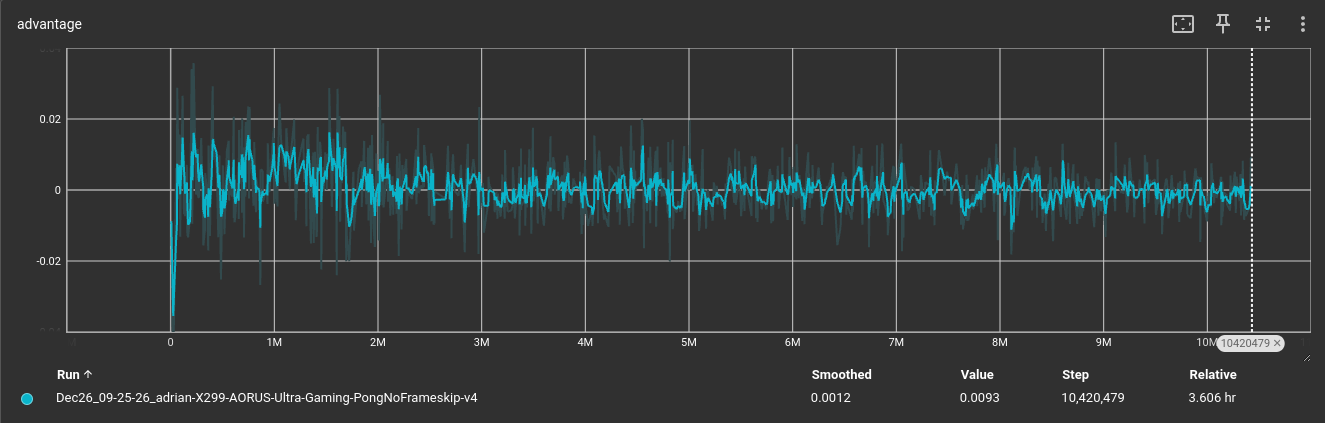
\includegraphics[width=\textwidth]{pictures/A2C_advantage.png}
        \caption{Wykres przedstawiający wartość przewagi modelu A2C}
    \end{figure}
    Wartość przewagi reprezentuje różnicę między wartością konkretnej akcji w danym stanie a uogólnioną wartością tego stanu. Odgrywa kluczową rolę w uczeniu A2C, ponieważ pomaga ograniczyć wariancję w estymacji wartości akcji.
    Wahania w początkowej fazie świadczą o tym, że agent wciąż uczy się oceniać akcje w poszczególnych stanach, co skutkuje zmiennością przewag. Stopniowa stabilizacja sugeruje, że model z czasem poprawnie identyfikuje wartości akcji, co przekłada się na lepszą politykę w dłuższej perspektywie.
    \\ \\ 
    \begin{figure}[H]
        \centering
        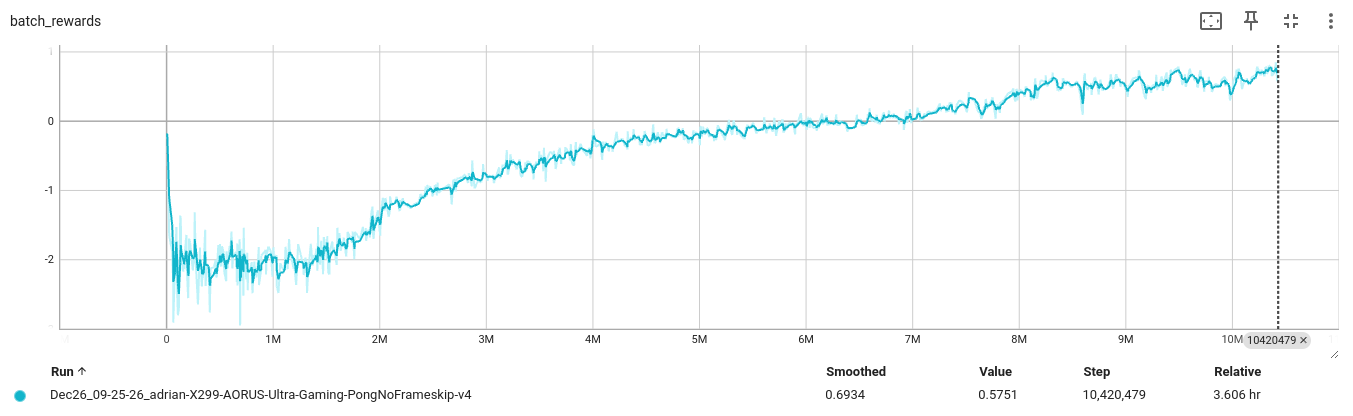
\includegraphics[width=\textwidth]{pictures/A2C_batch_rewards.png}
        \caption{Wykres przedstawiający średnią wartość paczki modelu A2C}
    \end{figure}
    Ilustruje uśrednione nagrody osiągane przez agenta w kolejnych epizodach:
    Początkowy wzrost wskazuje na szybkie dostosowywanie się modelu do wymagań środowiska. Stały wzrost wartości nagród w dalszej fazie sugeruje, że agent coraz lepiej rozumie otoczenie i opracowuje skuteczniejsze taktyki gry.
    \\ \\ 
    \begin{figure}[H]
        \centering
        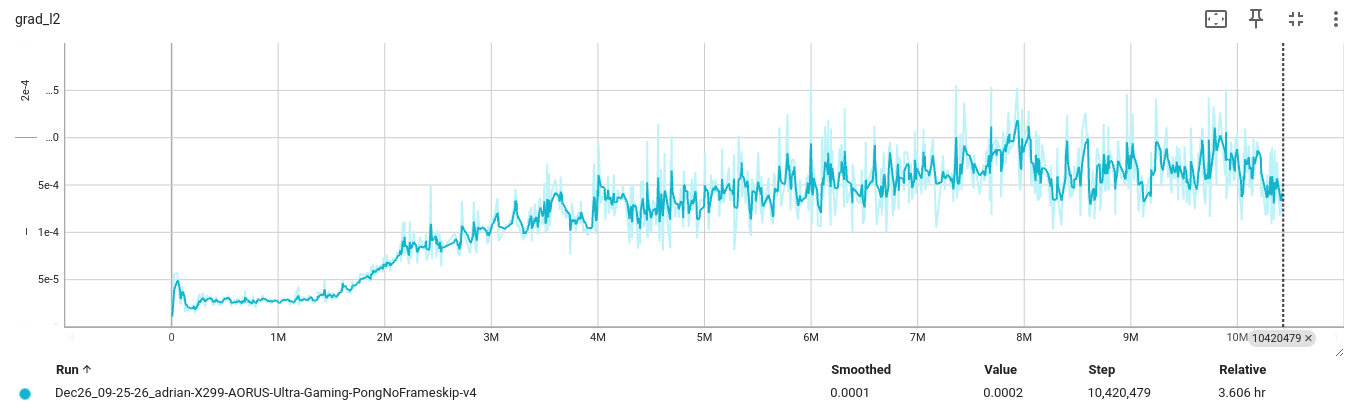
\includegraphics[width=\textwidth]{pictures/A2C_grad_l2.png}
        \caption{Wykres przedstawiający wielkosc normy gradientu L2 dla modelu A2C}
    \end{figure}
    Norma L2 gradientów określa siłę aktualizacji parametrów modelu. Zbyt duże wartości mogą prowadzić do niestabilności lub znacznych fluktuacji wag.  Zbyt małe wartości utrudniają osiągnięcie konwergencji.Zaobserwowana stabilizacja norm gradientów w trakcie treningu świadczy o prawidłowo przeprowadzanym procesie optymalizacji.
    \\ \\ 
    \begin{figure}[H]
        \centering
        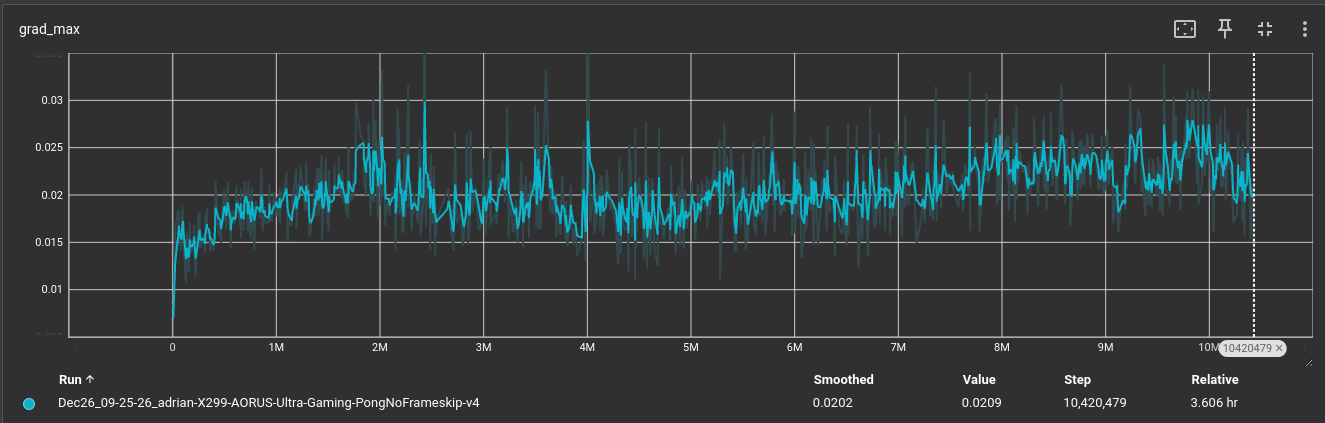
\includegraphics[width=\textwidth]{pictures/A2C_grad_max.png}
        \caption{Wykres przedstawiający gradient maksymalny modelu A2C}
    \end{figure}
    Maksymalne wartości gradientów wskazują na bardziej znaczące zmiany parametrów podczas trenowania modelu. Stabilizacja ich w późniejszym procesie treningu sugeruje, iż model zaczyna osiągać równowagę w uczeniu oraz dostosowywaniu się do środowiska.
    \\ \\ 
    \begin{figure}[H]
        \centering
        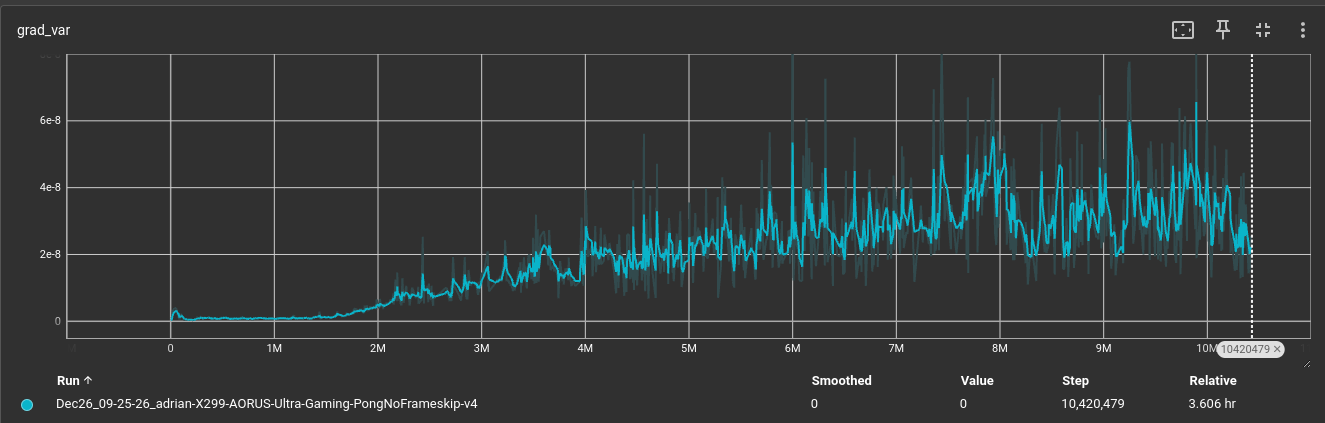
\includegraphics[width=\textwidth]{pictures/A2C_grad_var.png}
        \caption{Wykres przedstawiający wariancję gradnientu modelu A2C}
    \end{figure}
    Wariancja gradientów obrazuje, jak bardzo zróżnicowane są gradienty w kolejnych aktualizacjach. Wzrost wariancji może świadczyć o intensywnym poszukiwaniu nowych, lepszych strategii. Stopniowy wzrost pod koniec treningu oznacza większą pewność modelu co do wypracowanych rozwiązań.
    \\ \\ 
    \begin{figure}[H]
        \centering
        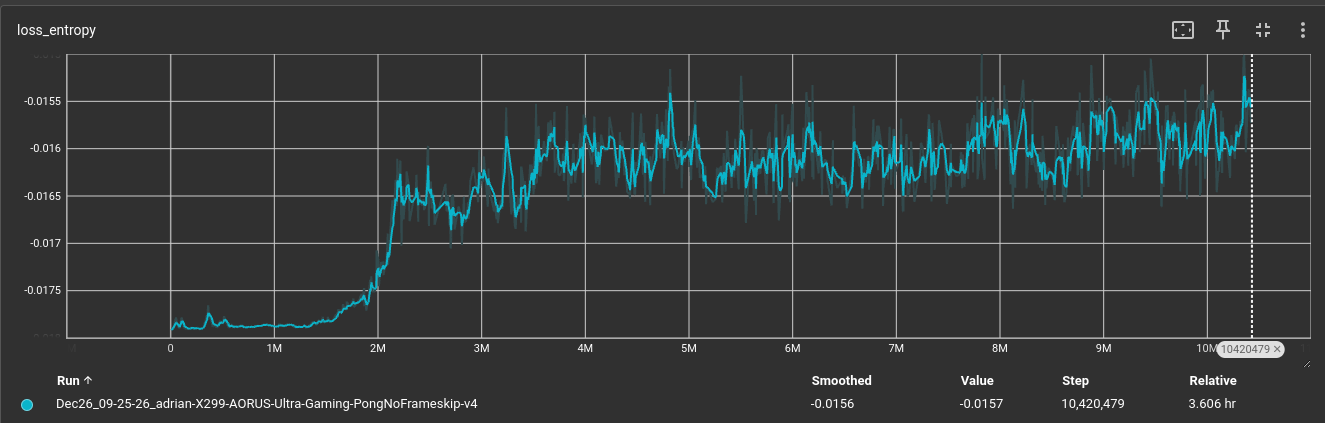
\includegraphics[width=\textwidth]{pictures/A2C_loss_entropy.png}
        \caption{Wykres przedstawiający stratę entropii modelu A2C}
    \end{figure}
    Strata entropii mierzy poziom eksploracji w polityce agenta.
    Zmniejszająca się wartość entropii w procesie treningu modelu
    oznacza, że model staje się bardziej pewny w procesie podejmowania decyzji. Początkowo wysoka entropia wskazuje na eksplorację,
    następnie jej spadek w późniejszych etapach wskazuje na stabilizację polityki.
    Zasadniczo oznacza to, że podczas gdy polityka zaczyna się zmieniać, agent staje się coraz bardziej pewny akcji, które wykonuje.
    \\ \\ 
    \begin{figure}[H]
        \centering
        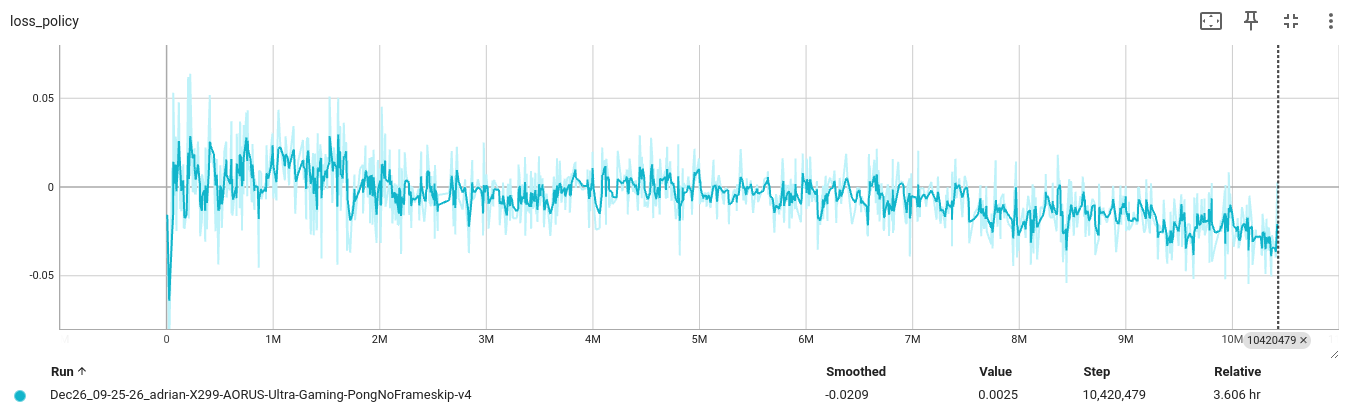
\includegraphics[width=\textwidth]{pictures/A2C_loss_policy.png}
        \caption{Wykres przedstawiający stratę polityki modelu A2C}
    \end{figure}
    Przedstawia, w jakim tempie i w jakim kierunku dostosowują się parametry sieci aktora. 
    Znaczne zmiany w początkowej fazie typowe dla etapu intensywnej eksploracji i poszukiwania lepszych akcji.
    Stabilizacja w późniejszej fazie świadczy o zbliżaniu się do polityki zoptymalizowanej (lub lokalnie zoptymalizowanej). Jest to zjawisko pozytywne.
    \\ \\ 
    \begin{figure}[H]
        \centering
        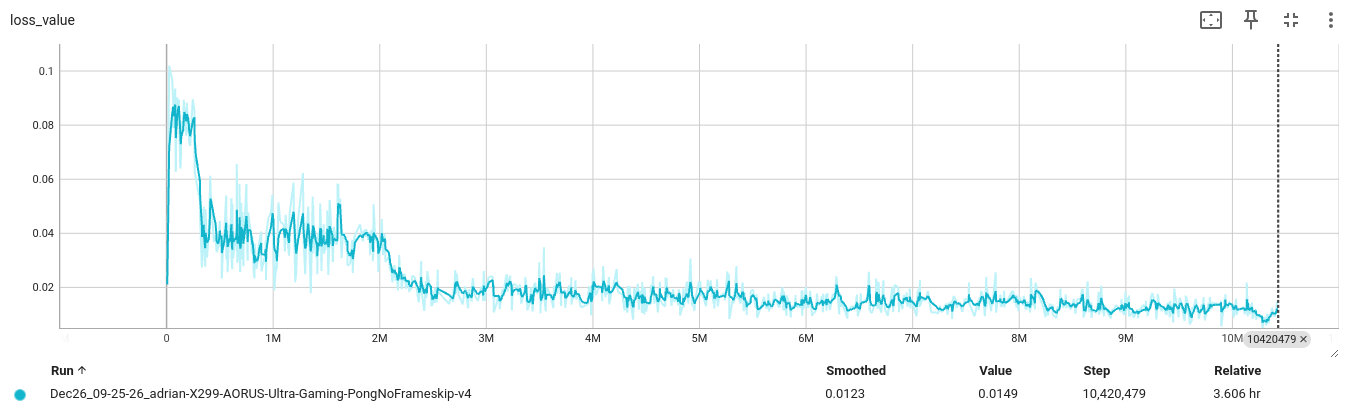
\includegraphics[width=\textwidth]{pictures/A2C_loss_value.png}
        \caption{Wykres przedstawiający stratę wartości modelu A2C}
    \end{figure}
    Odzwierciedla różnicę między przewidywaną a rzeczywistą wartością stanu. Systematyczny spadek: wskazuje, że sieć krytyka coraz trafniej przewiduje wartość stanu.
    Poprawa estymacji wskazuje na lepiej wyestymowana wartość stanu umożliwia szybszą i bardziej precyzyjną aktualizację polityki.
    \\ \\ 
    \begin{figure}[H]
        \centering
        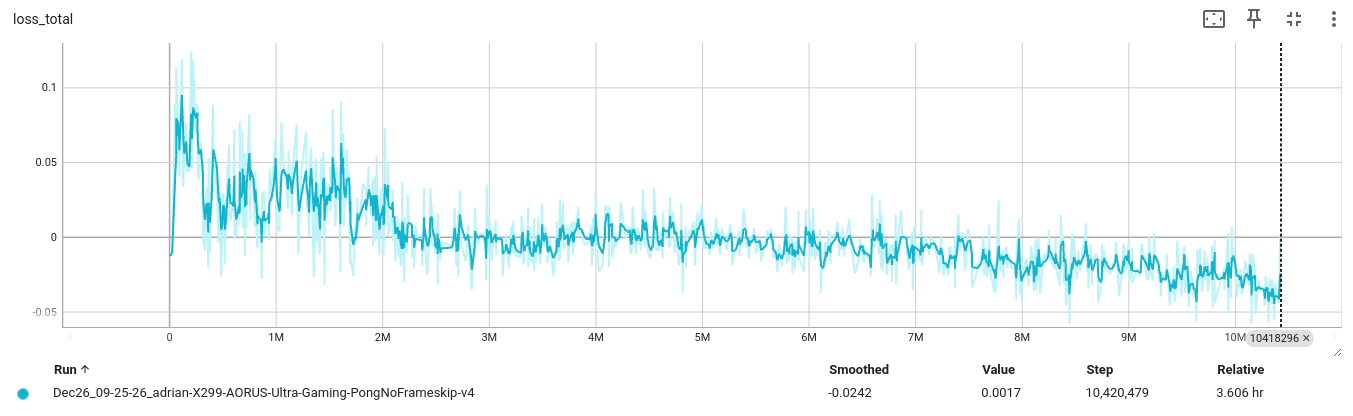
\includegraphics[width=\textwidth]{pictures/A2C_loss_total.png}
        \caption{Wykres przedstawiający stratę całkowitą modelu A2C}
    \end{figure}
    Łączna strata to kombinacja strat polityki, wartości oraz entropii. Ma za zadanie
    ona odzwierciedlić ogólny koszt optymalizacji procesu.
    Malejący trend pokazuje, że algorytm skutecznie minimalizuje błąd funkcji kosztu.
    Stabilizacja pod koniec sugeruje zbliżanie się do równowagi między eksploracją a eksploatacją.
    \\ \\ 
    \begin{figure}[H]
        \centering
        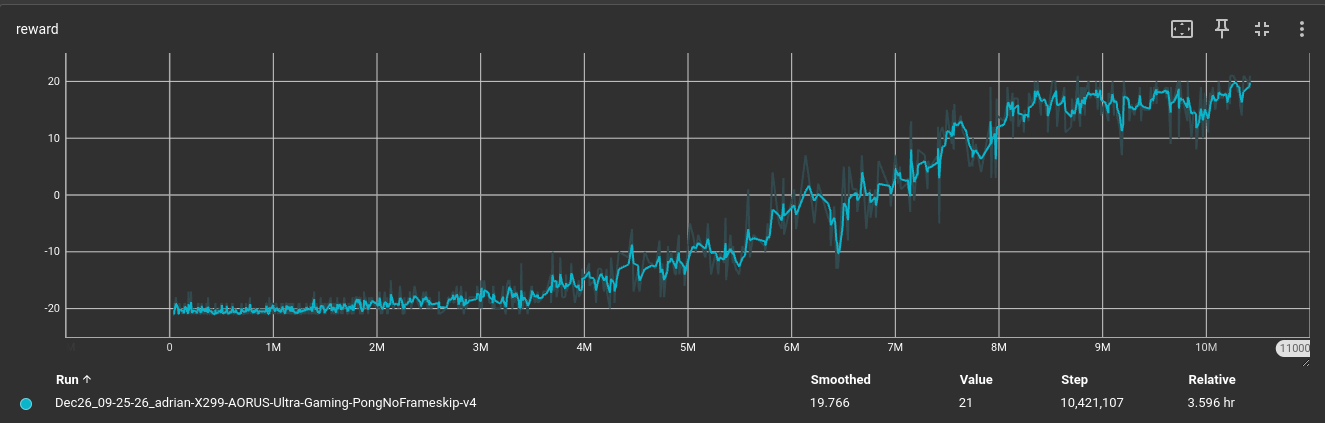
\includegraphics[width=\textwidth]{pictures/A2C_reward.png}
        \caption{Wykres przedstawiający średnią nagrodę modelu A2C}
    \end{figure}
    Wartość nagrody dla każdego kolejnego epizodu procesu uczenia ilustruje efektywność modelu.
    Niskie wartości na początku są typowe dla fazy eksploracji i braku wyuczonej strategii. Stopniowy wzrost świadczy o ciągłym ulepszaniu polityki, co skutkuje wyższą liczbą punktów zdobywanych przez agenta.
    Osiągnięcie maksymalnych wartości (ok. +21) oznacza pełne opanowanie środowiska Pong (lub osiągnięcie wyniku zbliżonego do perfekcji).
    \subsection{Struktura projektu}
    Diagram UML przedstawiony na rys. 5.13 ilustruje przykładową implementację algorytmu Advantage Actor-Critic (A2C). Diagram koncentruje się na głównych klasach i ich wzajemnych relacjach, nie wchodząc w szczegółowe opisy wszystkich metod wewnętrznych. Najważniejsze elementy projektu to:
    \begin{figure}[H]
        \centering
        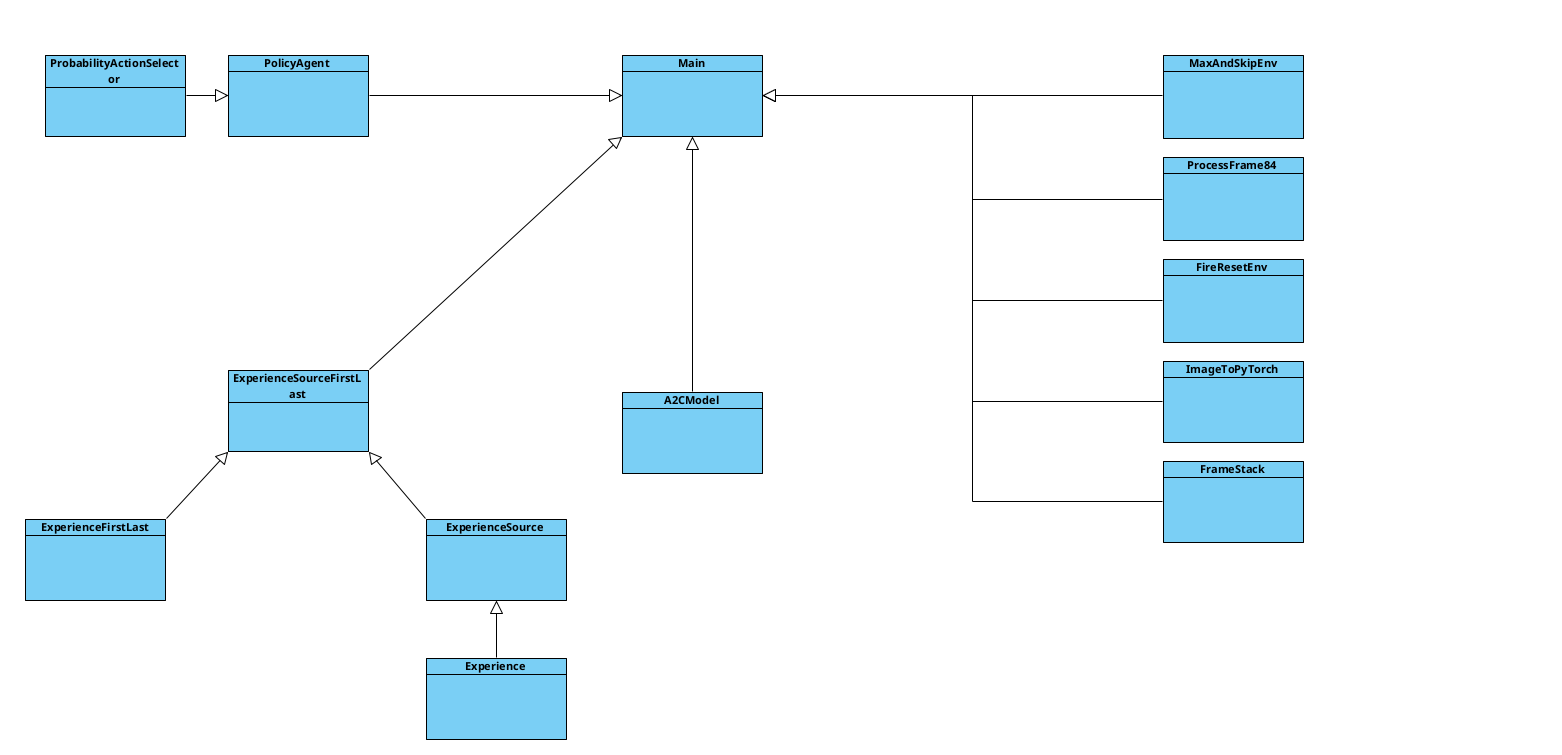
\includegraphics[width=\textwidth]{pictures/A2C_diagram.png}
        \caption{Diagram stuktury projektu modelu A2C}
    \end{figure}
    \begin{itemize}
        \item Main - w tym module inicjalizowane jest środowisko i koordynowany zostaje proces uczenia. Tworzone są tu liczne obiekty (m.in. A2CModel, PolicyAgent, ExperienceSourceFirstLast), a następnie uruchamiana jest główna pętla treningowa. Podczas tej pętli agent iteracyjnie gromadzi doświadczenia, oddziałując ze środowiskiem gry Pong, zaś sieć (A2C) jest regularnie aktualizowana przy użyciu optymalizatora (funkcja Adam). Moduł odpowiada również za zapisywanie wyników oraz ewentualne wczytywanie wytrenowanych modeli.
        \item A2CModel - jest to sieć neuronowa łącząca w jednej architekturze funkcje aktora i krytyka. Sieć konwolucyjna służy do przetwarzania surowych obrazów pochodzących z gry. Rozdzielenie wyjść (dla warstwy aktora oraz krytyka) umożliwia równoczesne wyznaczanie prawdopodobieństw akcji i estymację ich oczekiwanej wartości.
        \item PolicyAgent - klasa pełniąca rolę pośrednika między środowiskiem a modelem. Na podstawie bieżącej obserwacji otrzymuje z sieci A2C rozkład prawdopodobieństwa wybrania poszczególnych akcji i dokonuje ostatecznego wyboru ruchu, który zostaje wykonany w środowisku.
        \item ProbabilityActionSelector - obiekt ten otrzymuje rozkład prawdopodobieństwa akcji wygenerowany przez sieć i na tej podstawie losuje konkretną akcję do wykonania. Rozwiązanie takie wprowadza element stochastyczności, wspierając eksplorację środowiska i redukując ryzyko zbyt wczesnej stabilizacji strategii.
        \item Experience - struktura przechowująca informacje dotyczące pojedynczego kroku w środowisku: obserwacji, wybranej akcji oraz otrzymanej nagrody. Upraszcza zarządzanie historią rozgrywki i umożliwia przejrzyste gromadzenie danych.
        \item ExperienceFirstLast - rozszerzona wersja rekordu doświadczenia, w której oprócz standardowych informacji przechowywane jest także odniesienie do stanu końcowego. Ułatwia to obliczanie zdyskontowanych sum nagród w podejściu A2C, szczególnie przydatnych do treningu krytyka.
        \item ExperienceSource - podstawowy generator strumienia doświadczeń. Scala on dane z wielu środowisk oraz integruje działania agenta, zarządzając uruchamianiem kolejnych epizodów, gromadzeniem sygnałów zwrotnych oraz przygotowywaniem sekwencji kroków niezbędnych do dalszej obróbki.
        \item ExperienceSourceFirstLast - specjalizowana wersja generatora, wykorzystująca strukturę ExperienceFirstLast. Pozwala na pobieranie niewielkich sekwencji kroków, jednocześnie automatycznie obliczając zdyskontowane sumy nagród. Zabieg ten wpisuje się w schemat A2C, gdzie istotne jest uwzględnienie wartości przyszłych nagród.
        \item MaxAndSkipEnv - mechanizm pozwalający pominąć część klatek i jednocześnie zsumować odpowiadające im nagrody. Wykorzystuje on maksymalne wartości pikseli z dwóch ostatnich obserwacji, co prowadzi do redukcji liczby kroków przetwarzanych podczas treningu i tym samym zwiększa efektywność obliczeń.
        \item FireResetEnv - odpowiada za inicjalizację rozgrywki przez wymuszenie akcji FIRE (oraz ewentualnie innej) na początku każdego epizodu. Dzięki temu mechanizmowi agent może od razu rozpocząć właściwą interakcję z grą.
        \item ProcessFrame84 - ten komponent przetwarza pojedynczą klatkę na obraz w odcieniach szarości oraz skaluje go do rozmiaru 84x84. Pozwala to znacząco zmniejszyć wymiarowość danych wejściowych, co korzystnie wpływa na szybkość i stabilność treningu
        \item ImageToPyTorch - zadaniem ImageToPyTorch jest zmiana kolejności wymiarów klatki z postaci (wysokość, szerokość, kanały) na (kanały, wysokość, szerokość).Ułatwia to dalsze przetwarzanie obrazu w bibliotece PyTorch, w której standardem jest inna konwencja wymiarów tensora.
        \item FrameStack - utrzymuje stos kilku ostatnich klatek (np. czterech) i traktuje je jako pojedynczą obserwację, co pomaga sieci uchwycić krótkoterminową dynamikę obiektów w grze (ruch piłki czy paletki).
    \end{itemize}
    Opisana struktura umożliwia agentowi otrzymywanie przetworzonych danych o stanie gry, na podstawie których sieć neuronowa A2C (działająca w roli aktora i krytyka) wyznacza optymalne akcje. Trening polega na iteracyjnym aktualizowaniu wag w celu minimalizacji błędu estymacji wartości oraz maksymalizacji skumulowanej nagrody zdobywanej przez agenta. Połączenie architektury aktor - krytyk ze starannie zorganizowanym mechanizmem gromadzenia obserwacji zapewnia stabilną optymalizację i umożliwia efektywne opanowanie gry Pong.
    \\ \\ 
    Pełną implementację kodu można znaleźć na repozytorium github \cite{A2C}
    Kod został zainspirowany rozwiązaniami przedstawionymi w książce Maxima Lapana \cite{lapan2020deep} i dostosowany do najnowszych wersji bibliotek.
    \subsection{Tabela z wynikami dla różnych hiperparametrów}
    \begin{table}[H]
        \centering
        \begin{tabular}{>{\bfseries}l>{\centering\arraybackslash}m{1cm}>{\centering\arraybackslash}m{2cm}>{\centering\arraybackslash}m{2cm}>{\arraybackslash}m{3cm}}
        \toprule
        \textbf{Hiperparametr} & \textbf{Zmiana} & \textbf{Czas} & \textbf{Liczba kroków } & \textbf{Uwagi} \\
        \midrule
        $\gamma$ & 0.95 & $ \sim 3 $ godziny & $ \sim 8500000 $ & Szybsza konwergencja, mniejsze nagrody. \\
        \addlinespace
        BATCH\_SIZE & 64 & $ \sim 2 $ godziny & $ \sim 6000000 $ & Mniej stabilne wyniki, szybsze uczenie. \\
        \addlinespace
        BATCH\_SIZE & 32 & $ \sim 1,7 $ godziny & $ \sim 4300000 $ & Mniej stabilne wyniki, szybsze uczenie. \\
        \addlinespace
        REPLAY\_SIZE & 50,000 & $ \sim 2,5 $ godziny & $ \sim 1100000$ & Większa różnorodność danych, dłuższy czas treningu. \\
        \addlinespace
        LEARNING\_RATE & 0.002 & 5500000 & ~1,8 godziny & Szybsza konwergencja, większe wahania wyników. \\
        \addlinespace
        LEARNING\_RATE & 0.003 & N/A & N/A & Brak konwegencji. \\
        \addlinespace
        ENDROPY\_BETA & 0.03 & $\sim 4,5 $ godziny & $ \sim 13500000 $  & Większa eksploatacja kosztem eksploracji, dłuższy czas konwergencji. \\
        \bottomrule
        \end{tabular}
        \caption{Wyniki eksperymentów dla różnych hiperparametrów.}
        \label{tab:wyniki}
        \end{table}
    \subsection{Wnioski}
    Przedstawiony algorytm A2C pozwala na pomyślne wytrenowanie agenta w środowisku Pong i uzyskanie optymalnej lub zbliżonej do optymalnej polityki gry. W porównaniu z algorytmem DQN, A2C oferuje bardziej stabilny proces treningowy, co w dużej mierze wynika z równoległego wykorzystywania wielu środowisk i regularyzacji entropii. Architektura aktor-krytyk pozwala na efektywniejsze zarządzanie informacjami zwrotnymi, dzięki czemu agent w mniejszym stopniu ulega przetrenowaniu i szybciej przystosowuje się do wymagań zadania.
    \section{Podsumowanie}
    Głównym celem przeprowadzonych badań była analiza efektywności wybranych algorytmów uczenia przez wzmacnianie w kontekście gry Pong, która stanowi często stosowane środowisko testowe dla metod sztucznej inteligencji. W ramach pracy przedstawiono kluczowe założenia teoretyczne dotyczące procesów decyzyjnych Markowa oraz zaprezentowano znaczenie równań Bellmana w procesie optymalizacji polityki.

    Praktyczna część prac koncentrowała się na porównaniu dwóch podejść: Deep Q-Learning (DQN) oraz Advantage Actor-Critic (A2C). Dokonano szczegółowego omówienia ich architektur i sposobu treningu, a także wpływu doboru hiperparametrów na stabilność i szybkość konwergencji. Wyniki eksperymentów wskazały, że DQN, choć w wielu przypadkach pozwala osiągać zadowalające rezultaty, bywa podatny na przetrenowanie. Z kolei A2C, dzięki architekturze aktor-krytyk, okazał się bardziej stabilny i skuteczny w osiąganiu długoterminowych celów.

    W trakcie badań zidentyfikowano również znaczenie właściwego dostrajania hiperparametrów (takich jak współczynnik uczenia czy entropia), które okazało się niezbędnym warunkiem do uzyskania wysokich wyników. Odpowiednia konfiguracja parametrów bywa równie ważna jak sam wybór algorytmu i często decyduje o ostatecznej efektywności metody.

    Uzyskane rezultaty potwierdzają, że algorytmy uczenia przez wzmacnianie stanowią obiecujące narzędzie do rozwiązywania problemów decyzyjnych, jednak ich wydajność silnie zależy od właściwego przygotowania środowiska, umiejętnego doboru architektury sieciowej oraz przemyślanej selekcji hiperparametrów. Uzyskane wnioski mogą być wykorzystane jako punkt wyjścia do dalszych badań nad bardziej zaawansowanymi podejściami, takimi jak Asynchronous Avantage Actor-Critic (A3C) \cite{mnih2016a3c} czy Proximal Policy Optimization (PPO) \cite{schulman2017proximal}, i ich potencjalnym zastosowaniem nie tylko w grach komputerowych, lecz także w robotyce czy analizie danych.

    Dzięki połączeniu wiedzy teoretycznej z weryfikacją praktyczną przedstawione w niniejszej pracy wyniki umożliwiły uzyskanie spójnego obrazu efektywności algorytmów uczenia przez wzmacnianie w środowisku Pong i wskazały najważniejsze kierunki dalszych poszukiwań badawczych.
    \section{Bibliografia}
    \printbibliography
\end{document} 